\documentclass[11pt,a4paper]{article}
% SCRS/2026/143 — diagnostic appendices only (WG submission).
% Main framework paper body is not included; compile from 3diags/:
%   pdflatex SCRS_2026_143_appendices.tex
%   bibtex SCRS_2026_143_appendices
%   pdflatex SCRS_2026_143_appendices.tex
%   pdflatex SCRS_2026_143_appendices.tex
%
% Or: Rscript appendices/R/render-wg-appendices.R --compile

\usepackage[margin=2.5cm]{geometry}
\usepackage{setspace}
\usepackage{authblk}
\usepackage{graphicx}
\usepackage{booktabs}
\usepackage{multirow}
\usepackage{amssymb}
\usepackage{hyperref}
\usepackage{natbib}
\usepackage{float}
\usepackage{rotating}

\graphicspath{{figs/}{appendices/figs/}}
\hypersetup{hypertexnames=false}
\setstretch{1.0}
\parskip=6pt
\parindent=0pt
\pagestyle{empty}

\title{\textbf{Diagnostic Appendices for SCRS/2026/143}\\
\large Internal, External, and Robustness Diagnostics\\
\large Shortfin Mako Shark --- 2026 Working Group Assessment Runs}

\author[1]{Laurence T. Kell}
\author[2]{Massimiliano Cardinale}

\affil[1]{Centre for Environmental Policy, Imperial College London}
\affil[2]{Swedish University of Agricultural Sciences, Department of Aquatic Resources}

\date{}

\begin{document}
\maketitle

\section*{Purpose}

These appendices accompany \textbf{SCRS/2026/143} (\emph{From Fitted to Fit-for-Purpose: Intertwining the Strands of Stock Assessment Diagnostics}). The main document presents the three-strand framework and a small set of illustrative figures; \textbf{this document holds the full reproducible diagnostic workflow} for the updated 2026 working-group SS3 scenarios.

The main paper text is frozen for conversion to a peer-reviewed journal article. \textbf{All new analyses from the 2026 assessment runs belong here}---likelihood profiles, retrospectives, hindcasts, process-error panels, ensemble summaries, and interpretation---without modifying the framework narrative in SCRS/2026/143.

% Scope note for SCRS/2026/143 working-group appendices (auto-updated at render).

This appendix documents diagnostic outputs for the \textbf{2026 shortfin mako working-group assessment runs}. It is intended to supplement document \textbf{SCRS/2026/143}, which presents the three-strand diagnostic \textit{framework} with selected examples in the main body. Detailed tables, figures, and reproducible checks are maintained here so that new analyses from updated SS3 runs can be added without revising the main paper (which will be developed separately as a peer-reviewed journal article).

Generic computation resides in R packages (\texttt{sstruth}, \texttt{diags}, \texttt{r4ss}, \texttt{ss3diags}); case-study wiring and this LaTeX shell live in the \texttt{3diags} repository. Re-render after placing converged scenarios under the assessment base directory and running the appendix pipeline documented in \texttt{appendices/README.md}.

% 2026 ICCAT shark WG SS3 runs (P:/rfmo/iccat/2026/shark/Analysis/ss3).

\begin{table}[H]
\centering
\small
\caption{Shortfin mako SS3 scenarios and sensitivity runs used for the diagnostic checklist (Table~\ref{tab:diag-checklist}). Base runs are the principal scenarios; sensitivity runs are grouped under the Sens columns in the checklist.}
\label{tab:sma-scenario-runs}
\begin{tabular}{llp{7.5cm}}
\toprule
Scenario & Role & SS3 run directory (under \texttt{ss3/}) \\
\midrule
1 & Base & \texttt{Scenario\_1/Sc1\_Base} \\
1 & Sens & \texttt{Scenario\_1/Sc1\_SensA\_InitF0p05}, \texttt{Scenario\_1/Sc1\_SensB\_InitF0p005}, \texttt{Scenario\_1/Sc1\_SensC\_oldM\_newH}, \texttt{Scenario\_1/Sc1\_SensD\_includeCondAgeAtLength} \\
\addlinespace
2 & Base & \texttt{Scenario\_2/Scn02\_base} \\
2 & Sens & \texttt{Scenario\_2/Scn02\_SensA\_InitF\_0p05}, \texttt{Scenario\_2/Scn02\_SensB\_InitF\_0p005}, \texttt{Scenario\_2/Scn02\_SensC\_oldM\_newH} \\
\addlinespace
3 & Base & \texttt{Scenario\_3/Sc3\_Base} \\
3 & Sens & \texttt{Scenario\_3/Sc3\_SensA\_InitF0p05}, \texttt{Scenario\_3/Sc3\_SensB\_InitF0p005}, \texttt{Scenario\_3/Sc3\_SensC\_oldM\_newH}, \texttt{Scenario\_3/Sc3\_SensD\_excludeCondAgeAtLength} \\
\bottomrule
\end{tabular}
\end{table}


\begin{sidewaystable}[!p]
\centering
\small
\caption{Minimum diagnostics checklist for SS3 shortfin mako scenarios and sensitivities (2026 ICCAT shark WG). A tick (\checkmark) indicates that the diagnostic has been applied and documented; a dash (--) indicates not applied or not documented. Run directories are listed in Table~\ref{tab:sma-scenario-runs}.}
\label{tab:diag-checklist}
\begin{tabular}{llcccccc}
\toprule
 & & \multicolumn{2}{c}{Scenario 1} & \multicolumn{2}{c}{Scenario 2} & \multicolumn{2}{c}{Scenario 3} \\
\cmidrule(lr){3-4}\cmidrule(lr){5-6}\cmidrule(lr){7-8}
Strand & Diagnostic & Base & Sens & Base & Sens & Base & Sens \\
\midrule
\multirow{8}{*}{Internal}
 & Convergence: Hessian inverts, max gradient reported & \checkmark & \checkmark & \checkmark & \checkmark & \checkmark & \checkmark \\
 & Parameters at/near bounds listed & \checkmark & -- & \checkmark & -- & \checkmark & -- \\
 & High parameter correlations identified & \checkmark & -- & \checkmark & -- & \checkmark & -- \\
 & Selectivity and length-comp residual diagnostics (RMSE, runs) & \checkmark & -- & \checkmark & -- & \checkmark & -- \\
 & CPUE residual diagnostics (joint residuals, RMSE, runs) & \checkmark & -- & \checkmark & -- & \checkmark & -- \\
 & Effective sample size diagnostics (Francis / McAllister--Ianelli) & \checkmark & -- & \checkmark & -- & \checkmark & -- \\
 & Likelihood profile for $\log R_0$ (data vs prior) & \checkmark & -- & \checkmark & -- & \checkmark & -- \\
 & Jitter test for global convergence & \checkmark & -- & \checkmark & -- & \checkmark & -- \\
\midrule
\multirow{4}{*}{External}
 & Maturity--selectivity / fecundity--selectivity overlays & \checkmark & -- & \checkmark & -- & \checkmark & -- \\
 & Comparison of biomass and CPUE trends (survey perception) & \checkmark & -- & \checkmark & -- & \checkmark & -- \\
 & Age-structure response to exploitation (numbers-at-age patterns) & \checkmark & -- & \checkmark & -- & \checkmark & -- \\
 & External life-history consistency (growth, $M$, steepness) & \checkmark & -- & \checkmark & -- & \checkmark & -- \\
\midrule
\multirow{7}{*}{Robustness}
 & Leave-one-out CPUE (single index inclusion/exclusion) & \checkmark & -- & \checkmark & -- & \checkmark & -- \\
 & ASPM / ASPMdev (indices only, fixed selectivity) & \checkmark & -- & \checkmark & -- & \checkmark & -- \\
 & Retrospective patterns (Mohn's $\rho$) & \checkmark & -- & \checkmark & -- & \checkmark & -- \\
 & Hindcast prediction skill (HCXval, MASE) & \checkmark & -- & \checkmark & -- & \checkmark & -- \\
 & Alternative $M$ and steepness (original vs modified PW) & -- & \checkmark & -- & \checkmark & -- & \checkmark \\
 & Alternative initial $F$ prior & -- & \checkmark & -- & \checkmark & -- & \checkmark \\
 & CAAL growth sensitivity (Scenario 3) & -- & -- & -- & -- & \checkmark & \checkmark \\
\bottomrule
\end{tabular}
\end{sidewaystable}



\newpage
\tableofcontents
\newpage

\appendix
\section{Internal Diagnostics and Reproducible Workflow}
\label{app:internal}

Internal diagnostics evaluate whether the fitted model is consistent with its likelihood,
parameterisation, and data inputs. This appendix provides a reproducible structure for
detailed case-study reporting. Generic computation should live in R packages; case-study
scripts should load inputs, call package functions, record software versions, and write
tables and figures into the content files below.

\subsection{Required R Packages}

\begin{table}

\caption{\label{tab:internal-libraries}Required R packages for internal diagnostics.}
\centering
\begin{tabular}[t]{llll}
\toprule
package & role & tier & installed\\
\midrule
knitr & Knit template; format LaTeX tables & core & 1.51\\
r4ss & Read SS3 output; summarise convergence and likelihood components & run\_code & 1.53.0\\
sstruth & curveSS, diagSS, ssU, ssLen, ssRunSummary, residual plots & run\_code & 0.0.0.9020\\
diags & CPUE diagnostic summaries via sstruth::ssU & run\_code & 2.2.1\\
ggplot2 & Likelihood, residual, and recruitment-deviation figures & run\_code & 4.0.3\\
\addlinespace
reshape2 & Data reshaping for diagnostic plots & run\_code & 1.4.5\\
ss3diags & SSrunstest and ssruns\_sig3; CPUE runs-test plots with 3-sigma limits & run\_code & 1.10.2\\
FLRebuild & Fallback curveSS if sstruth unavailable & planned & 0.1.0\\
ss3om & Fallback readFLSss3 via readTruth (optional) & planned & 0.5.3.9004\\
\bottomrule
\end{tabular}
\end{table}



\subsection{Inputs}

Record the accepted model run, principal sensitivities, software versions, and data
objects used to create this appendix.

\begin{table}

\caption{\label{tab:internal-inputs}Internal diagnostics inputs.}
\centering
\begin{tabular}[t]{ll}
\toprule
item & value\\
\midrule
Assessment ID & sma-ss3-2026\\
Model class & SS3\\
SS base directory & P:/rfmo/iccat/2026/shark/Analysis/ss3\\
Scenarios & Scenario\_1/Sc1\_Base, Scenario\_2/Scn02\_base, Scenario\_3/Sc3\_Base\\
Reference scenario & Scenario\_1/Sc1\_Base\\
\addlinespace
SS version & 3.30\\
R version & 4.4.2\\
r4ss & 1.53.0\\
ss3diags & 1.10.2\\
sstruth & 0.0.0.9020\\
\addlinespace
diags & 2.2.1\\
FLRebuild & 0.1.0\\
ss3om & 0.5.3.9004\\
Run code & TRUE\\
\bottomrule
\end{tabular}
\end{table}



\subsection{Standard Checks}

The minimum internal checklist should include:

\begin{itemize}
  \item convergence status, maximum gradient, Hessian status, and parameters near bounds;
  \item likelihood components and evidence for conflicts among data sources;
  \item residual diagnostics for indices and composition data;
  \item effective sample size diagnostics for composition data;
  \item likelihood profiles or equivalent information-content diagnostics for advice-relevant quantities;
  \item recruitment deviations and whether stock--recruitment assumptions are informed by data;
  \item process-error diagnostics: residuals versus time, biomass, ACF, and distributional properties (Appendix~\ref{app:internal}, process-error outputs).
\end{itemize}

% Internal diagnostic checks.

\begin{table}

\caption{\label{tab:internal-convergence}Convergence and Hessian summary by scenario.}
\centering
\begin{tabular}[t]{lrrrrrr}
\toprule
scenario & n\_params & total\_ll & max\_grad & log\_det\_hessian & n\_iterations & n\_warnings\\
\midrule
Scenario-1 & 92 & 515.254 & 5.67e-05 & 134.9 & 801 & 7\\
Scenario-2 & 100 & 485.295 & 1.06e-05 & 160.9 & 863 & 6\\
Scenario-3 & 109 & 1164.320 & 9.18e-05 & 173.2 & 1061 & 6\\
\bottomrule
\end{tabular}
\end{table}

\begin{table}

\caption{\label{tab:internal-ll-components}Likelihood components for the reference scenario.}
\centering
\begin{tabular}[t]{llrr}
\toprule
  & component & log\_likelihood & lambda\\
\midrule
5 & Length\_comp & 613.162 & NA\\
4 & Survey & -88.782 & NA\\
6 & Recruitment & -10.025 & 1\\
9 & Parm\_priors & 0.772 & 1\\
8 & Forecast\_Recruitment & 0.111 & 1\\
\addlinespace
10 & Parm\_softbounds & 0.015 & NA\\
2 & Catch & 0.000 & NA\\
3 & Equil\_catch & 0.000 & NA\\
7 & InitEQ\_Regime & 0.000 & 1\\
11 & Parm\_devs & 0.000 & 1\\
\addlinespace
12 & Crash\_Pen & 0.000 & 1\\
\bottomrule
\end{tabular}
\end{table}

% No estimated parameters within 2 percent of bounds (reference scenario).

\begin{table}

\caption{\label{tab:internal-advice-pars}Advice-relevant parameters and asymptotic standard errors (reference scenario).}
\centering
\begin{tabular}[t]{llrrrrlr}
\toprule
  & Label & Value & Phase & Min & Max & Status & se\\
\midrule
SR\_autocorr & SR\_autocorr & 0.000000 & -4 & -5.00 & 5.00 & NA & NA\\
SR\_LN(R0) & SR\_LN(R0) & 5.528090 & 1 & 2.30 & 13.82 & OK & 0.126584\\
SR\_regime & SR\_regime & 0.000000 & -4 & -5.00 & 5.00 & NA & NA\\
SR\_sigmaR & SR\_sigmaR & 0.283103 & -4 & 0.20 & 1.90 & NA & NA\\
SR\_surv\_Beta & SR\_surv\_Beta & 3.000000 & -4 & 0.01 & 10.00 & NA & NA\\
\addlinespace
SR\_surv\_zfrac & SR\_surv\_zfrac & 0.372000 & -4 & 0.01 & 1.00 & NA & NA\\
\bottomrule
\end{tabular}
\end{table}

\begin{table}

\caption{\label{tab:internal-comp-ess}Length-composition effective sample size summary by fleet (sstruth::ssLen).}
\centering
\begin{tabular}[t]{lrrrlrrrrrrlrlllllrrrl}
\toprule
  & Data\_type & Fleet & Recommend\_var\_adj & \# & N & Npos & min\_Nsamp & max\_Nsamp & mean\_Nsamp\_in & mean\_Nsamp\_adj & mean\_Nsamp\_DM & err\_method & err\_index & par1 & val1 & par2 & val2 & mean\_effN & HarMean & Curr\_Var\_Adj & Fleet\_name\\
\midrule
3618 & 4 & 1 & 1.595300 & \# & 22 & 22 & 4.10135 & 26.88660 & 22.63640 & 10.31550 & NA & 0 & NA & multinomial & NA & NA & NA & 73.2504 & 36.1118 & 0.455705 & F01\_EU\_SPN\\
3619 & 4 & 2 & 3.348320 & \# & 13 & 13 & 5.75133 & 9.58555 & 11.07690 & 7.07856 & NA & 0 & NA & multinomial & NA & NA & NA & 40.8450 & 37.0890 & 0.639037 & F02\_EU\_POR\\
3620 & 4 & 3 & 4.379130 & \# & 15 & 15 & 7.08631 & 18.22190 & 10.53330 & 10.66320 & NA & 0 & NA & multinomial & NA & NA & NA & 49.4968 & 46.1268 & 1.012330 & F03\_JPN\\
3621 & 4 & 4 & 1.711010 & \# & 4 & 4 & 2.57489 & 6.11536 & 11.50000 & 3.70140 & NA & 0 & NA & multinomial & NA & NA & NA & 22.9236 & 19.6766 & 0.321861 & F04\_CTP\\
3622 & 4 & 5 & 6.092490 & \# & 24 & 24 & 10.60390 & 37.87100 & 13.95830 & 21.14460 & NA & 0 & NA & multinomial & NA & NA & NA & 103.6380 & 85.0410 & 1.514840 & F05\_USA\\
\addlinespace
3623 & 4 & 6 & 3.428940 & \# & 14 & 14 & 3.09308 & 6.62804 & 10.28570 & 4.54494 & NA & 0 & NA & multinomial & NA & NA & NA & 50.2229 & 35.2691 & 0.441869 & F06\_CAN\\
3624 & 4 & 7 & 0.983769 & \# & 6 & 6 & 6.03750 & 34.21250 & 23.33330 & 23.47920 & NA & 0 & NA & multinomial & NA & NA & NA & 28.7302 & 22.9546 & 1.006250 & F07\_MOR\\
3625 & 4 & 8 & 5.842330 & \# & 22 & 22 & 21.53180 & 36.91160 & 9.18182 & 28.24300 & NA & 0 & NA & multinomial & NA & NA & NA & 61.8055 & 53.6432 & 3.075970 & F08\_MEX\\
3626 & 4 & 9 & 4.599110 & \# & 2 & 2 & 41.42290 & 55.23050 & 10.50000 & 48.32670 & NA & 0 & NA & multinomial & NA & NA & NA & 48.3984 & 48.2906 & 4.602540 & F09\_VEN\\
\bottomrule
\end{tabular}
\end{table}

\begin{table}

\caption{\label{tab:internal-ssu-summary}CPUE residual summary by fleet (sstruth::diagSS / ssU).}
\centering
\begin{tabular}[t]{lrrrr}
\toprule
name & n & mean\_abs\_residual & max\_abs\_std & runs\_p\\
\midrule
CPUE\_CTP & 11 & 0.59710 & NA & NA\\
CPUE\_EU\_POR & 25 & 0.25710 & NA & NA\\
CPUE\_EU\_SPN & 34 & 0.21250 & NA & NA\\
CPUE\_JPN\_1 & 14 & 0.13170 & NA & NA\\
CPUE\_JPN\_2 & 15 & 0.23190 & NA & NA\\
\addlinespace
CPUE\_MOR\_1 & 10 & 0.16010 & NA & NA\\
CPUE\_MOR\_2 & 2 & 0.08311 & NA & NA\\
CPUE\_USA & 32 & 0.28830 & NA & NA\\
CPUE\_USAlogbook & 30 & 0.19000 & NA & NA\\
\bottomrule
\end{tabular}
\end{table}

% SS3 run notes from sstruth::ssRunSummary:
% warning_excerpt: Note 1 Information: Max data length bin: 320  < max pop len bins: 380; so will accumulate larger pop len bins
% warning_excerpt: Warning 1 Adjustment: basis for HCR anchor was not set; setting to 2 to match default before 3.30.24
% warning_excerpt: Warning 2 : parm min for Lmin: 5 should not be less than population min length bin 35
% warning_excerpt: Note 2 Suggestion: Are you sure you want so few early recrdevs? Better to include in range of main recdevs 5
% warning_excerpt: Warning 3 : Setting in starter does not request all priors, and 40 parameters have priors and are not estimated, so their prior not included in obj_fun.
% warning_excerpt: Note 3 Information: A revised protocol for the Fcast_yr specification is available and recommended.
% warning_excerpt:  3 warnings  and 3 notes 

\begin{table}

\caption{\label{tab:internal-index-tuning}Index variance tuning and RMSE by CPUE fleet.}
\centering
\begin{tabular}[t]{lllllllll}
\toprule
  & Fleet & N & Npos & RMSE & Input+VarAdj+extra & VarAdj & New\_VarAdj & fleetname\\
\midrule
3455 & 12 & 34 & 34 & 0.315849 & 0.252706 & 0.132 & 0.327143 & CPUE\_EU\_SPN\\
3456 & 13 & 25 & 25 & 0.394276 & 0.43312 & 0 & -0.0388442 & CPUE\_EU\_POR\\
3457 & 14 & 14 & 14 & 0.175758 & 0.214643 & 0.163 & 0.287115 & CPUE\_JPN\_1\\
3458 & 15 & 15 & 15 & 0.286788 & 0.3668 & 0 & -0.0800123 & CPUE\_JPN\_2\\
3459 & 16 & 11 & 11 & 0.722256 & 0.326909 & 0.165 & 0.725347 & CPUE\_CTP\\
\addlinespace
3460 & 17 & 32 & 32 & 0.343423 & 0.273438 & 0.022 & 0.113985 & CPUE\_USA\\
3461 & 18 & 10 & 10 & 0.212431 & 0.2545 & 0.129 & 0.215931 & CPUE\_MOR\_1\\
3462 & 19 & 2 & 2 & 0.0831072 & 0.2005 & 0.01 & -0.0973928 & CPUE\_MOR\_2\\
3463 & 20 & 30 & 30 & 0.247158 & 0.210087 & 0.12 & 0.277072 & CPUE\_USAlogbook\\
\bottomrule
\end{tabular}
\end{table}

\begin{table}

\caption{\label{tab:internal-runs-test}CPUE residual runs-test summary by fleet (ss3diags::SSrunstest).}
\centering
\begin{tabular}[t]{lrlrrl}
\toprule
Index & runs.p & test & sigma3.lo & sigma3.hi & type\\
\midrule
CPUE\_EU\_SPN & 0.249 & Passed & -0.4816 & 0.4816 & cpue\\
CPUE\_EU\_POR & 0.272 & Passed & -0.7635 & 0.7635 & cpue\\
CPUE\_JPN\_1 & 0.013 & Failed & -0.3828 & 0.3828 & cpue\\
CPUE\_JPN\_2 & 0.092 & Passed & -0.8176 & 0.8176 & cpue\\
CPUE\_CTP & 0.475 & Passed & -2.0140 & 2.0140 & cpue\\
\addlinespace
CPUE\_USA & 0.145 & Passed & -0.6970 & 0.6970 & cpue\\
CPUE\_MOR\_1 & 0.103 & Passed & -0.5004 & 0.5004 & cpue\\
CPUE\_MOR\_2 & NA & Excluded & NA & NA & cpue\\
CPUE\_USAlogbook & 0.000 & Failed & -0.2873 & 0.2873 & cpue\\
\bottomrule
\end{tabular}
\end{table}

\begin{table}

\caption{\label{tab:internal-runs-qic}CPUE residual individual-chart runs tests by fleet (crossings and longest-run criteria).}
\centering
\begin{tabular}[t]{llrrrrlll}
\toprule
scenario & name & n.crossings & n.crossings.min & longest.run & longest.run.max & crossings & runs & Pass\\
\midrule
Scenario 1 & CPUE\_CTP & 5 & 2 & 4 & 6 & TRUE & TRUE & TRUE\\
Scenario 1 & CPUE\_EU\_POR & 11 & 6 & 3 & 7 & TRUE & TRUE & TRUE\\
Scenario 1 & CPUE\_EU\_SPN & 15 & 8 & 6 & 8 & TRUE & TRUE & TRUE\\
Scenario 1 & CPUE\_JPN\_1 & 3 & 3 & 5 & 6 & FALSE & TRUE & FALSE\\
Scenario 1 & CPUE\_JPN\_2 & 5 & 3 & 6 & 6 & TRUE & FALSE & FALSE\\
\addlinespace
Scenario 1 & CPUE\_MOR\_1 & 3 & 2 & 3 & 6 & TRUE & TRUE & TRUE\\
Scenario 1 & CPUE\_MOR\_2 & 1 & 0 & 1 & 3 & TRUE & TRUE & TRUE\\
Scenario 1 & CPUE\_USA & 13 & 7 & 6 & 7 & TRUE & TRUE & TRUE\\
Scenario 1 & CPUE\_USAlogbook & 3 & 7 & 12 & 7 & FALSE & FALSE & FALSE\\
\bottomrule
\end{tabular}
\end{table}

\begin{table}

\caption{\label{tab:internal-rec-sigma}Recruitment deviation summary statistics from SS3 report.}
\centering
\begin{tabular}[t]{lrrrrrrrrl}
\toprule
period & N\_devs & SD\_of\_devs & Var\_of\_devs & mean\_SE & mean\_SEsquared & sqrt\_sum\_of\_components & SD\_of\_devs\_over\_sigma\_R & sqrt\_sum\_over\_sigma\_R & alternative\_sigma\_R\\
\midrule
Main & 31 & 0.1805979 & 0.0326156 & 0.1971533 & 0.0391536 & 0.2678978 & 0.6379228 & 0.9462909 & 0.26789779814548\\
Early+Main & 36 & 0.1758351 & 0.0309180 & 0.2051770 & 0.0427470 & 0.2714129 & 0.6210994 & 0.9587074 & 0.271412929542226\\
Early+Main+Late & 39 & 0.1705995 & 0.0291042 & 0.2090008 & 0.0444819 & 0.2712676 & 0.6026058 & 0.9581939 & 0.271267571442131\\
\bottomrule
\end{tabular}
\end{table}

\begin{table}

\caption{\label{tab:internal-rec-rmse}Recruitment-deviation RMSE and Durbin-Watson diagnostics.}
\centering
\begin{tabular}[t]{lrrrrrr}
\toprule
ERA & N & RMSE & RMSE\textasciicircum{}2/sigmaR\textasciicircum{}2 & mean\_BiasAdj & est\_rho & Durbin-Watson\\
\midrule
main & 31 & 0.177661 & 0.393818 & 0.376244 & 0.602694 & 0.778993\\
early & 5 & 0.155099 & 0.300142 & 0.229362 & NA & NA\\
\bottomrule
\end{tabular}
\end{table}

\begin{table}

\caption{\label{tab:internal-profile-manifest}Likelihood-profile SS3 run manifest (M $\times$ SR\_surv\_Beta grid).}
\centering
\begin{tabular}[t]{rrlrl}
\toprule
M & beta & dir & total\_ll & ok\\
\midrule
0.500 & 0.5 & C:/active/scrs-papers/ss-ll/data/ICCAT\_2017\_Model\_Run\_3\_SSv330.23.02/00\_Model\_run\_files/0.5/0.5 & 83.2768 & TRUE\\
0.500 & 1.0 & C:/active/scrs-papers/ss-ll/data/ICCAT\_2017\_Model\_Run\_3\_SSv330.23.02/00\_Model\_run\_files/0.5/1 & 82.8158 & TRUE\\
0.500 & 1.5 & C:/active/scrs-papers/ss-ll/data/ICCAT\_2017\_Model\_Run\_3\_SSv330.23.02/00\_Model\_run\_files/0.5/1.5 & 82.4124 & TRUE\\
0.625 & 0.5 & C:/active/scrs-papers/ss-ll/data/ICCAT\_2017\_Model\_Run\_3\_SSv330.23.02/00\_Model\_run\_files/0.625/0.5 & 80.4027 & TRUE\\
0.625 & 1.0 & C:/active/scrs-papers/ss-ll/data/ICCAT\_2017\_Model\_Run\_3\_SSv330.23.02/00\_Model\_run\_files/0.625/1 & 79.9028 & TRUE\\
\addlinespace
0.625 & 1.5 & C:/active/scrs-papers/ss-ll/data/ICCAT\_2017\_Model\_Run\_3\_SSv330.23.02/00\_Model\_run\_files/0.625/1.5 & 79.4653 & TRUE\\
0.750 & 0.5 & C:/active/scrs-papers/ss-ll/data/ICCAT\_2017\_Model\_Run\_3\_SSv330.23.02/00\_Model\_run\_files/0.75/0.5 & 79.0489 & TRUE\\
0.750 & 1.0 & C:/active/scrs-papers/ss-ll/data/ICCAT\_2017\_Model\_Run\_3\_SSv330.23.02/00\_Model\_run\_files/0.75/1 & 78.5454 & TRUE\\
0.750 & 1.5 & C:/active/scrs-papers/ss-ll/data/ICCAT\_2017\_Model\_Run\_3\_SSv330.23.02/00\_Model\_run\_files/0.75/1.5 & 78.1602 & TRUE\\
0.875 & 0.5 & C:/active/scrs-papers/ss-ll/data/ICCAT\_2017\_Model\_Run\_3\_SSv330.23.02/00\_Model\_run\_files/0.875/0.5 & 78.5405 & TRUE\\
\addlinespace
0.875 & 1.0 & C:/active/scrs-papers/ss-ll/data/ICCAT\_2017\_Model\_Run\_3\_SSv330.23.02/00\_Model\_run\_files/0.875/1 & 78.1173 & TRUE\\
0.875 & 1.5 & C:/active/scrs-papers/ss-ll/data/ICCAT\_2017\_Model\_Run\_3\_SSv330.23.02/00\_Model\_run\_files/0.875/1.5 & 77.6292 & TRUE\\
1.000 & 0.5 & C:/active/scrs-papers/ss-ll/data/ICCAT\_2017\_Model\_Run\_3\_SSv330.23.02/00\_Model\_run\_files/1/0.5 & 78.5944 & TRUE\\
1.000 & 1.0 & C:/active/scrs-papers/ss-ll/data/ICCAT\_2017\_Model\_Run\_3\_SSv330.23.02/00\_Model\_run\_files/1/1 & 78.0832 & TRUE\\
1.000 & 1.5 & C:/active/scrs-papers/ss-ll/data/ICCAT\_2017\_Model\_Run\_3\_SSv330.23.02/00\_Model\_run\_files/1/1.5 & 77.6315 & TRUE\\
\addlinespace
1.125 & 0.5 & C:/active/scrs-papers/ss-ll/data/ICCAT\_2017\_Model\_Run\_3\_SSv330.23.02/00\_Model\_run\_files/1.125/0.5 & 78.8160 & TRUE\\
1.125 & 1.0 & C:/active/scrs-papers/ss-ll/data/ICCAT\_2017\_Model\_Run\_3\_SSv330.23.02/00\_Model\_run\_files/1.125/1 & 78.3617 & TRUE\\
1.125 & 1.5 & C:/active/scrs-papers/ss-ll/data/ICCAT\_2017\_Model\_Run\_3\_SSv330.23.02/00\_Model\_run\_files/1.125/1.5 & 77.9736 & TRUE\\
1.250 & 0.5 & C:/active/scrs-papers/ss-ll/data/ICCAT\_2017\_Model\_Run\_3\_SSv330.23.02/00\_Model\_run\_files/1.25/0.5 & 79.2123 & TRUE\\
1.250 & 1.0 & C:/active/scrs-papers/ss-ll/data/ICCAT\_2017\_Model\_Run\_3\_SSv330.23.02/00\_Model\_run\_files/1.25/1 & 78.8435 & TRUE\\
\addlinespace
1.250 & 1.5 & C:/active/scrs-papers/ss-ll/data/ICCAT\_2017\_Model\_Run\_3\_SSv330.23.02/00\_Model\_run\_files/1.25/1.5 & 78.5343 & TRUE\\
1.375 & 0.5 & C:/active/scrs-papers/ss-ll/data/ICCAT\_2017\_Model\_Run\_3\_SSv330.23.02/00\_Model\_run\_files/1.375/0.5 & 79.7198 & TRUE\\
1.375 & 1.0 & C:/active/scrs-papers/ss-ll/data/ICCAT\_2017\_Model\_Run\_3\_SSv330.23.02/00\_Model\_run\_files/1.375/1 & 79.4526 & TRUE\\
1.375 & 1.5 & C:/active/scrs-papers/ss-ll/data/ICCAT\_2017\_Model\_Run\_3\_SSv330.23.02/00\_Model\_run\_files/1.375/1.5 & 79.2327 & TRUE\\
1.500 & 0.5 & C:/active/scrs-papers/ss-ll/data/ICCAT\_2017\_Model\_Run\_3\_SSv330.23.02/00\_Model\_run\_files/1.5/0.5 & 80.7181 & TRUE\\
\addlinespace
1.500 & 1.0 & C:/active/scrs-papers/ss-ll/data/ICCAT\_2017\_Model\_Run\_3\_SSv330.23.02/00\_Model\_run\_files/1.5/1 & 80.6296 & TRUE\\
1.500 & 1.5 & C:/active/scrs-papers/ss-ll/data/ICCAT\_2017\_Model\_Run\_3\_SSv330.23.02/00\_Model\_run\_files/1.5/1.5 & 80.5685 & TRUE\\
\bottomrule
\end{tabular}
\end{table}



\subsection{Process Error and Stock--Recruitment Diagnostics}

Process-error diagnostics follow the four-panel structure described in Section~2.1 of the main text: temporal patterns (including regime-shift filters such as STARS), biomass-dependent bias, autocorrelation structure, and distributional properties. Where stock--recruitment relationships are fitted externally to assessment outputs, report whether uncertainty in SSB and recruitment was propagated; internal state-space formulations (e.g.\ SAM) should be distinguished from post-hoc fits to SS3 point estimates.

% Process-error diagnostic outputs (curveSS).

\begin{figure}[H]
  \centering
  \includegraphics[width=0.95\linewidth]{appendices/figs/internal/production-functions-scenarios.png}
  \caption{Production functions by SS3 scenario (curveSS; historical SSB--yield trajectory; Kobe quadrants, MSY, 40\% $B_\mathrm{max}$ path).}
  \label{fig:internal-production-functions-scenarios}
\end{figure}

\begin{figure}[H]
  \centering
  \includegraphics[width=0.95\linewidth]{appendices/figs/internal/kobe-phase-scenarios.png}
  \caption{Kobe phase plot by SS3 scenario (curveSS).}
  \label{fig:internal-kobe-phase-scenarios}
\end{figure}

\begin{figure}[H]
  \centering
  \includegraphics[width=0.92\linewidth]{appendices/figs/internal/pe-four-panel.png}
  \caption{Four-panel process-error diagnostics (curveSS).}
  \label{fig:internal-pe-four-panel}
\end{figure}


\subsection{Diagnostic Output}

Tables, figures, and code-generated summaries can be added to the file below as they
become available.

% Internal diagnostic figures and tables.

\begin{figure}[H]
  \centering
  \includegraphics[width=0.92\linewidth]{appendices/figs/internal/ss3-ts.png}
  \caption{SS3 scenario time series relative to MSY reference points (from curveSS).}
  \label{fig:internal-ss3-ts}
\end{figure}

\begin{figure}[H]
  \centering
  \includegraphics[width=0.92\linewidth]{appendices/figs/internal/ss3-pe-phase.png}
  \caption{Empirical production and curveSS yield curve versus spawning stock biomass.}
  \label{fig:internal-ss3-pe-phase}
\end{figure}

\begin{figure}[H]
  \centering
  \includegraphics[width=0.92\linewidth]{appendices/figs/internal/cpue-fit.png}
  \caption{Observed and expected CPUE indices (sstruth::diagSS).}
  \label{fig:internal-cpue-fit}
\end{figure}

\begin{figure}[H]
  \centering
  \includegraphics[width=0.92\linewidth]{appendices/figs/internal/cpue-residuals.png}
  \caption{CPUE residuals by fleet (sstruth::plotResiduals).}
  \label{fig:internal-cpue-residuals}
\end{figure}

\begin{figure}[H]
  \centering
  \includegraphics[width=0.92\linewidth]{appendices/figs/internal/cpue-std-residuals.png}
  \caption{Standardised CPUE residuals (sstruth::plotStdResiduals).}
  \label{fig:internal-cpue-std-residuals}
\end{figure}

\begin{figure}[H]
  \centering
  \includegraphics[width=0.95\linewidth]{appendices/figs/internal/cpue-runs-test.png}
  \caption{CPUE residual runs tests by fleet (individual-chart criteria; cf. figures.Rmd jara-runs).}
  \label{fig:internal-cpue-runs}
\end{figure}

\begin{figure}[H]
  \centering
  \includegraphics[width=0.95\linewidth]{appendices/figs/internal/cpue-runs-sig3.png}
  \caption{CPUE residual runs tests with 3-sigma limits (ss3diags::SSrunstest).}
  \label{fig:internal-cpue-runs-sig3}
\end{figure}

\begin{figure}[H]
  \centering
  \includegraphics[width=0.88\linewidth]{appendices/figs/internal/ll-components.png}
  \caption{Likelihood components for the reference scenario.}
  \label{fig:internal-ll-components}
\end{figure}

\begin{figure}[H]
  \centering
  \includegraphics[width=0.92\linewidth]{appendices/figs/internal/rec-devs.png}
  \caption{Recruitment deviations for the reference scenario.}
  \label{fig:internal-rec-devs}
\end{figure}

\begin{figure}[H]
  \centering
  \includegraphics[width=0.92\linewidth]{appendices/figs/internal/len-comp-residual-f1.png}
  \caption{Length-composition residuals, fleet 1 (sstruth::ssLen when available).}
  \label{fig:internal-len-comp-residual}
\end{figure}

\begin{figure}[H]
  \centering
  \includegraphics[width=0.88\linewidth]{appendices/figs/internal/ll-profile-total.png}
  \caption{Total log-likelihood profile over M and SR\_surv\_Beta fixed parameters.}
  \label{fig:internal-ll-profile-total}
\end{figure}

\begin{figure}[H]
  \centering
  \includegraphics[width=0.95\linewidth]{appendices/figs/internal/ll-profile-components.png}
  \caption{Likelihood-profile components by data source (M $\times$ SR\_surv\_Beta grid).}
  \label{fig:internal-ll-profile-components}
\end{figure}

\begin{figure}[H]
  \centering
  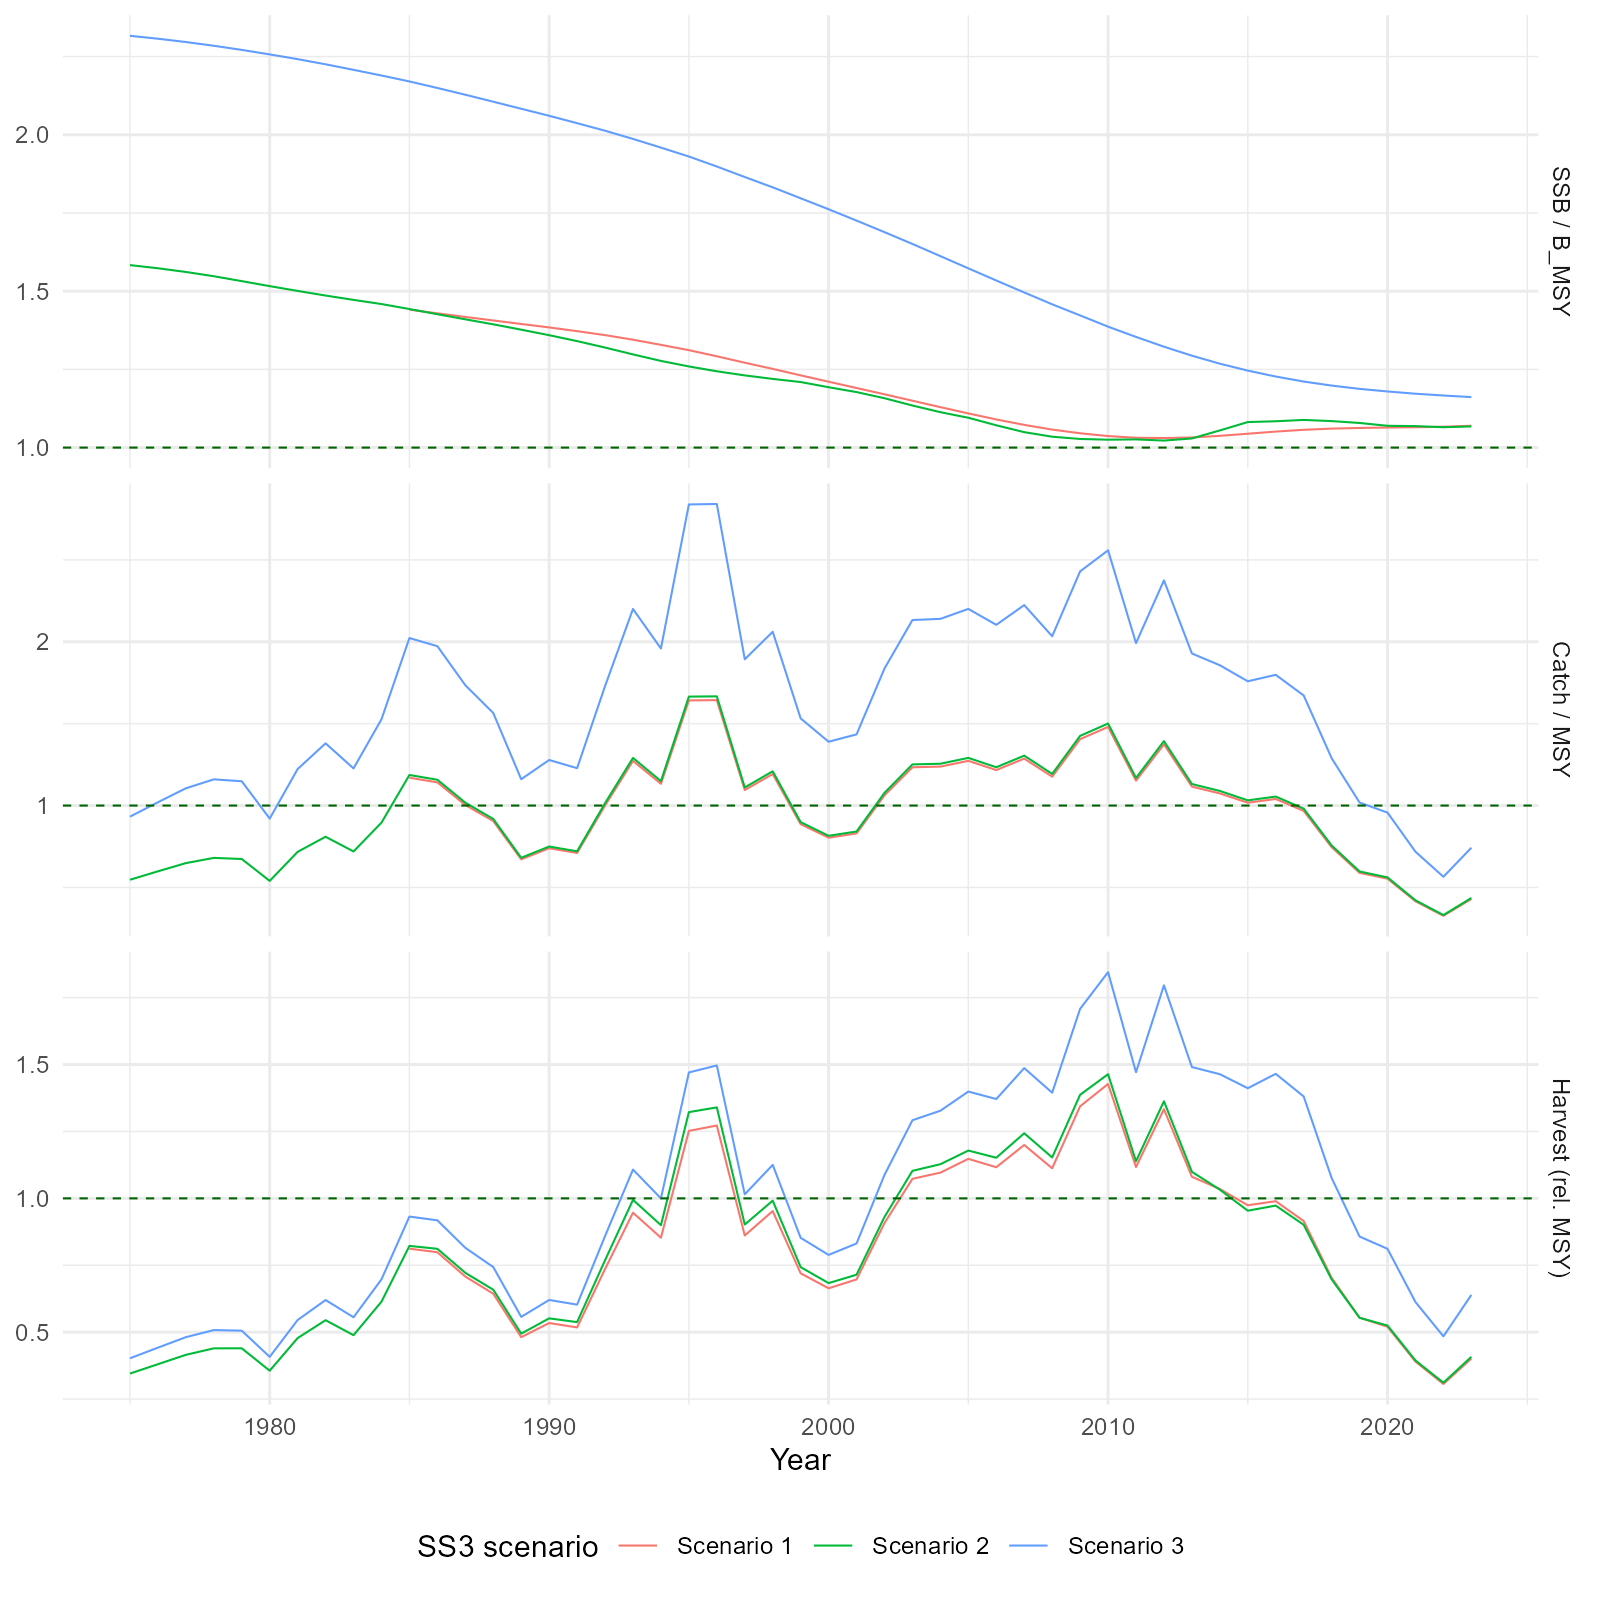
\includegraphics[width=0.92\linewidth]{figs/sma-fig-ts-1.png}
  \caption{sma fig ts 1}
  \label{fig:internal-sma-fig-ts-1}
\end{figure}

\begin{figure}[H]
  \centering
  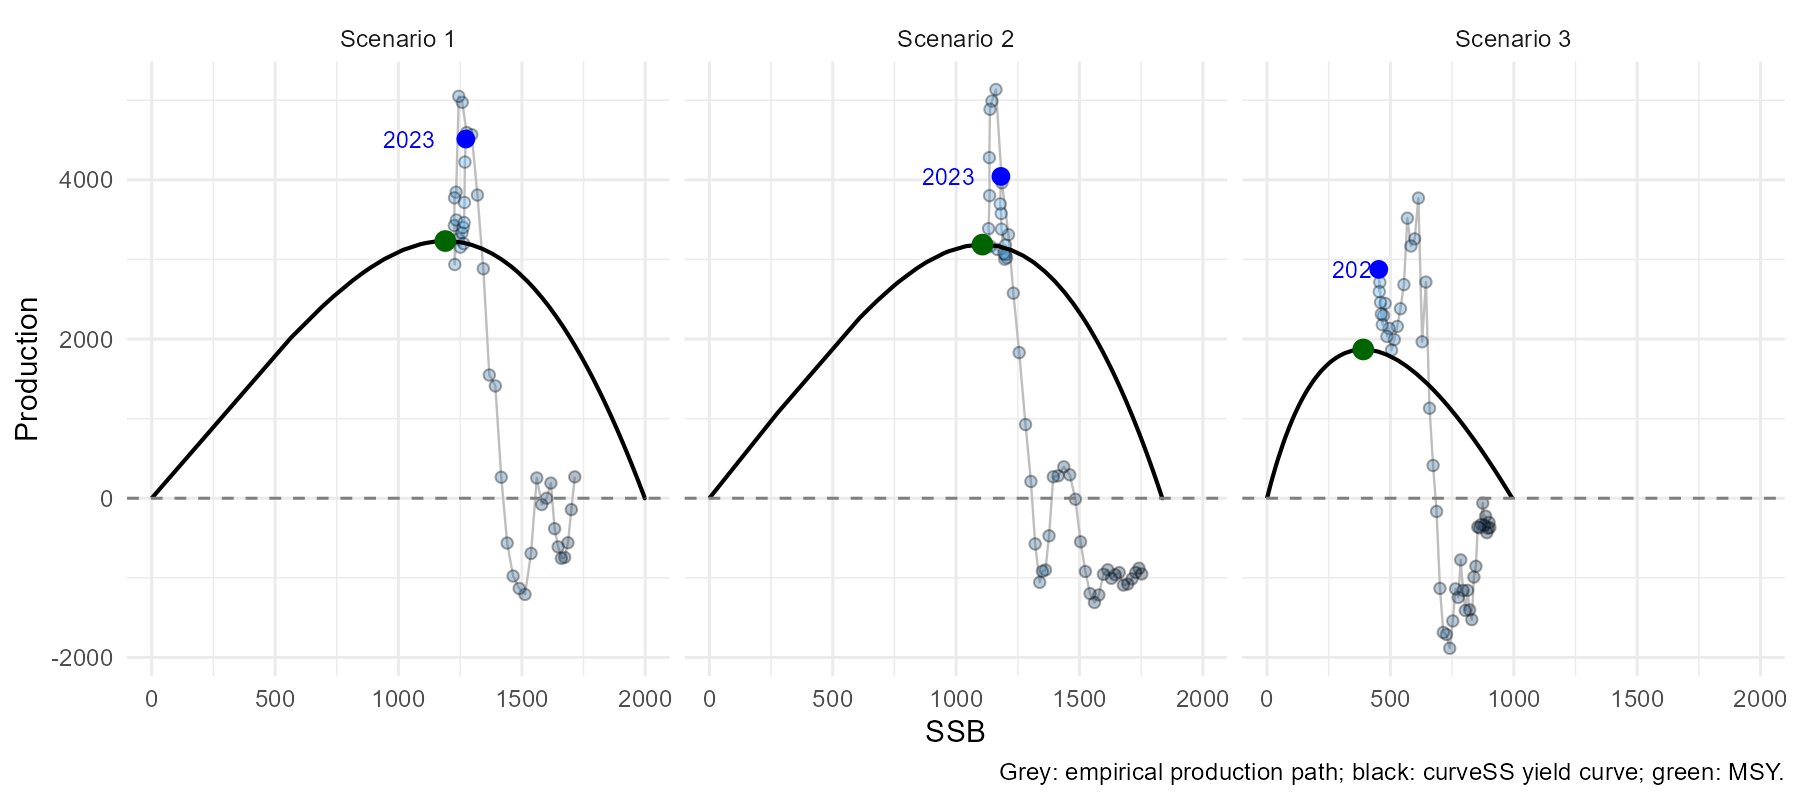
\includegraphics[width=0.92\linewidth]{figs/sma-fig-pe-phase-1.png}
  \caption{sma fig pe phase 1}
  \label{fig:internal-sma-fig-pe-phase-1}
\end{figure}

\begin{figure}[H]
  \centering
  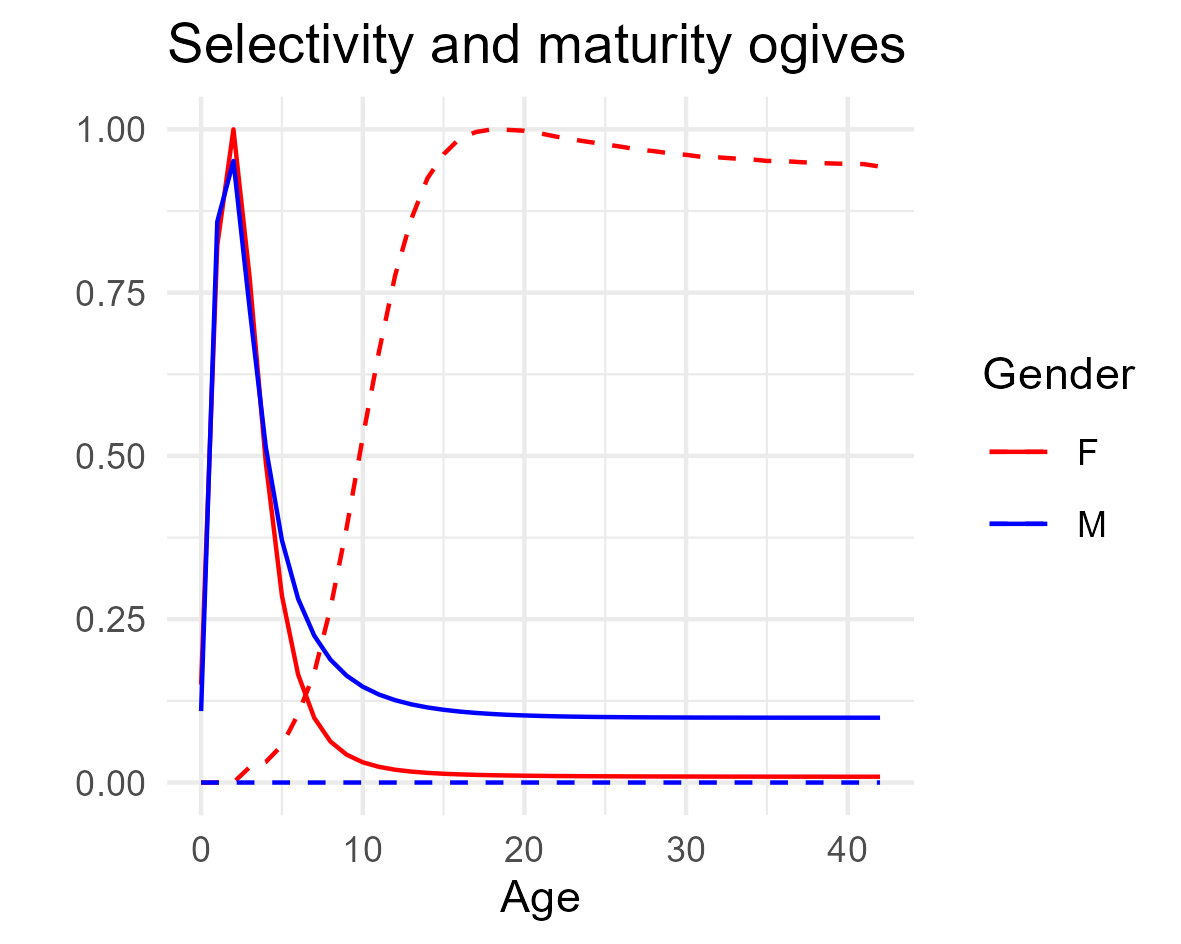
\includegraphics[width=0.92\linewidth]{figs/selmat.png}
  \caption{selmat}
  \label{fig:internal-selmat}
\end{figure}

\begin{figure}[H]
  \centering
  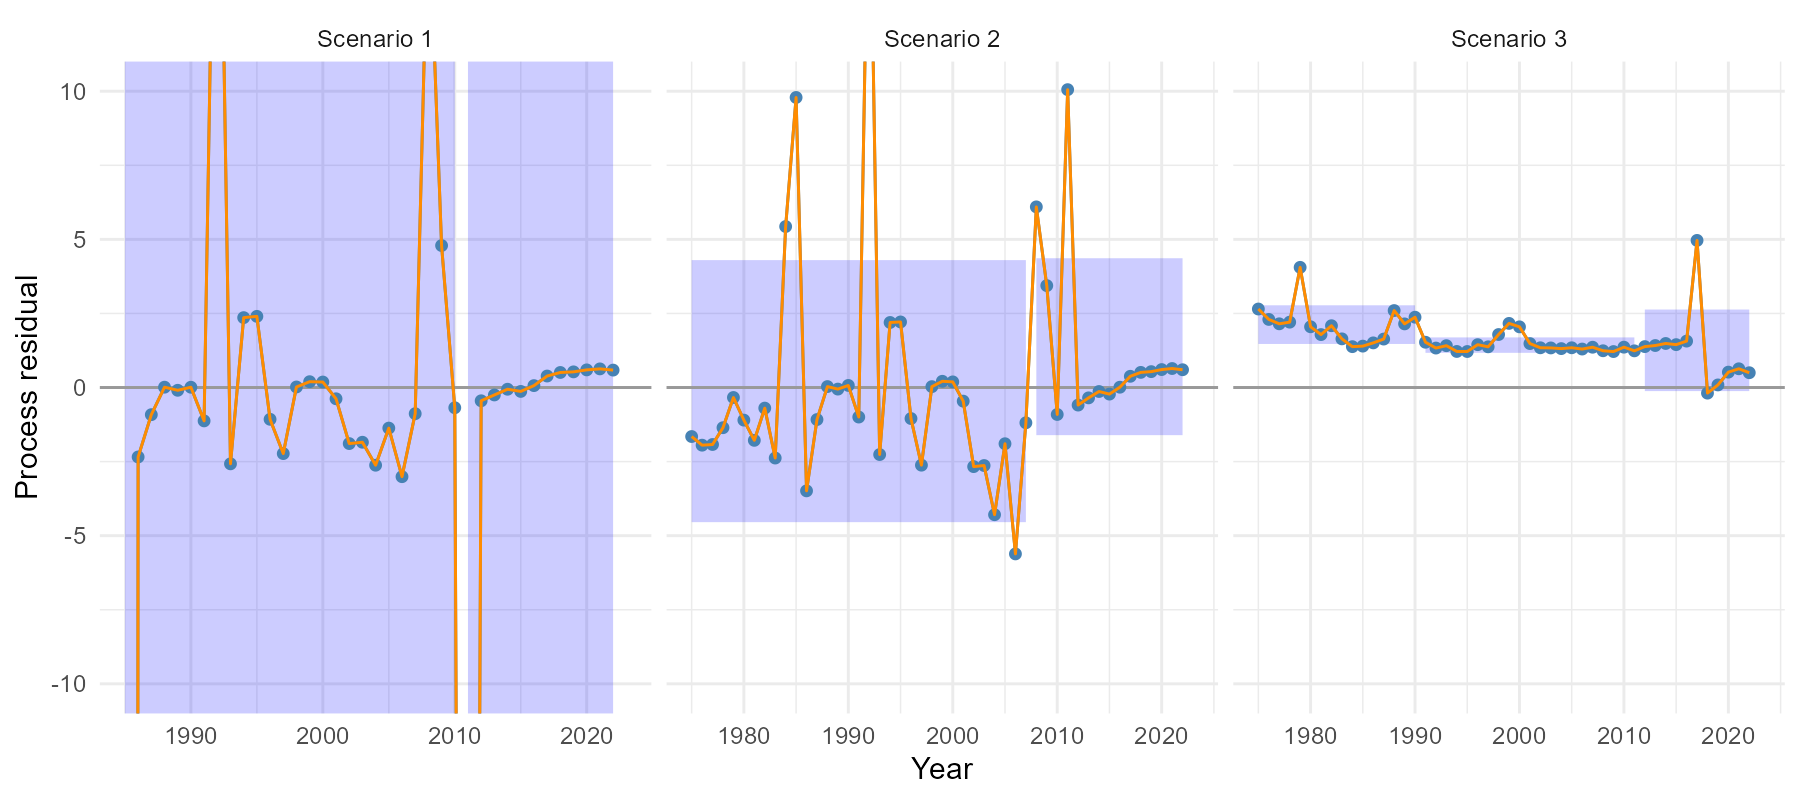
\includegraphics[width=0.92\linewidth]{figs/sma-fig-res-time-1.png}
  \caption{sma fig res time 1}
  \label{fig:internal-sma-fig-res-time-1}
\end{figure}

\begin{figure}[H]
  \centering
  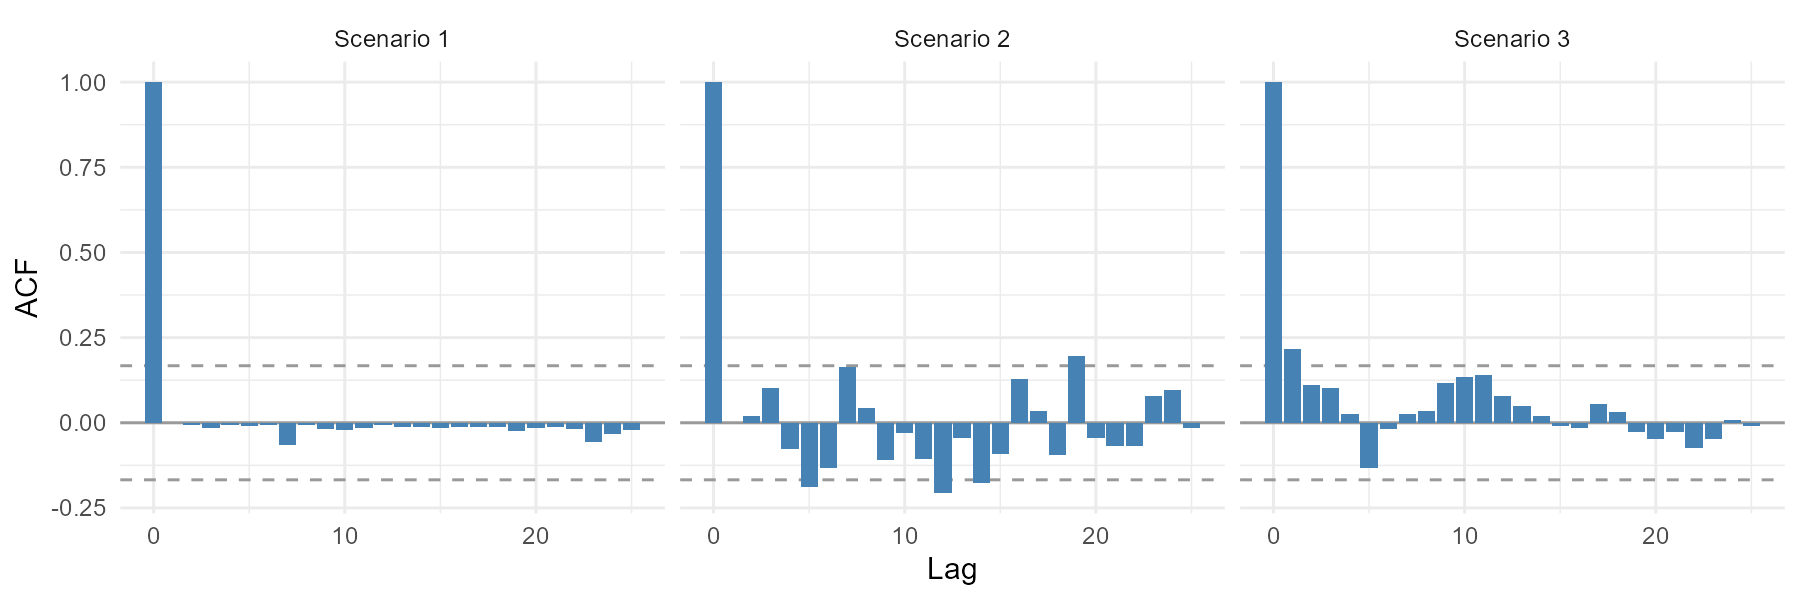
\includegraphics[width=0.92\linewidth]{figs/sma-fig-res-acf-1.png}
  \caption{sma fig res acf 1}
  \label{fig:internal-sma-fig-res-acf-1}
\end{figure}

\begin{figure}[H]
  \centering
  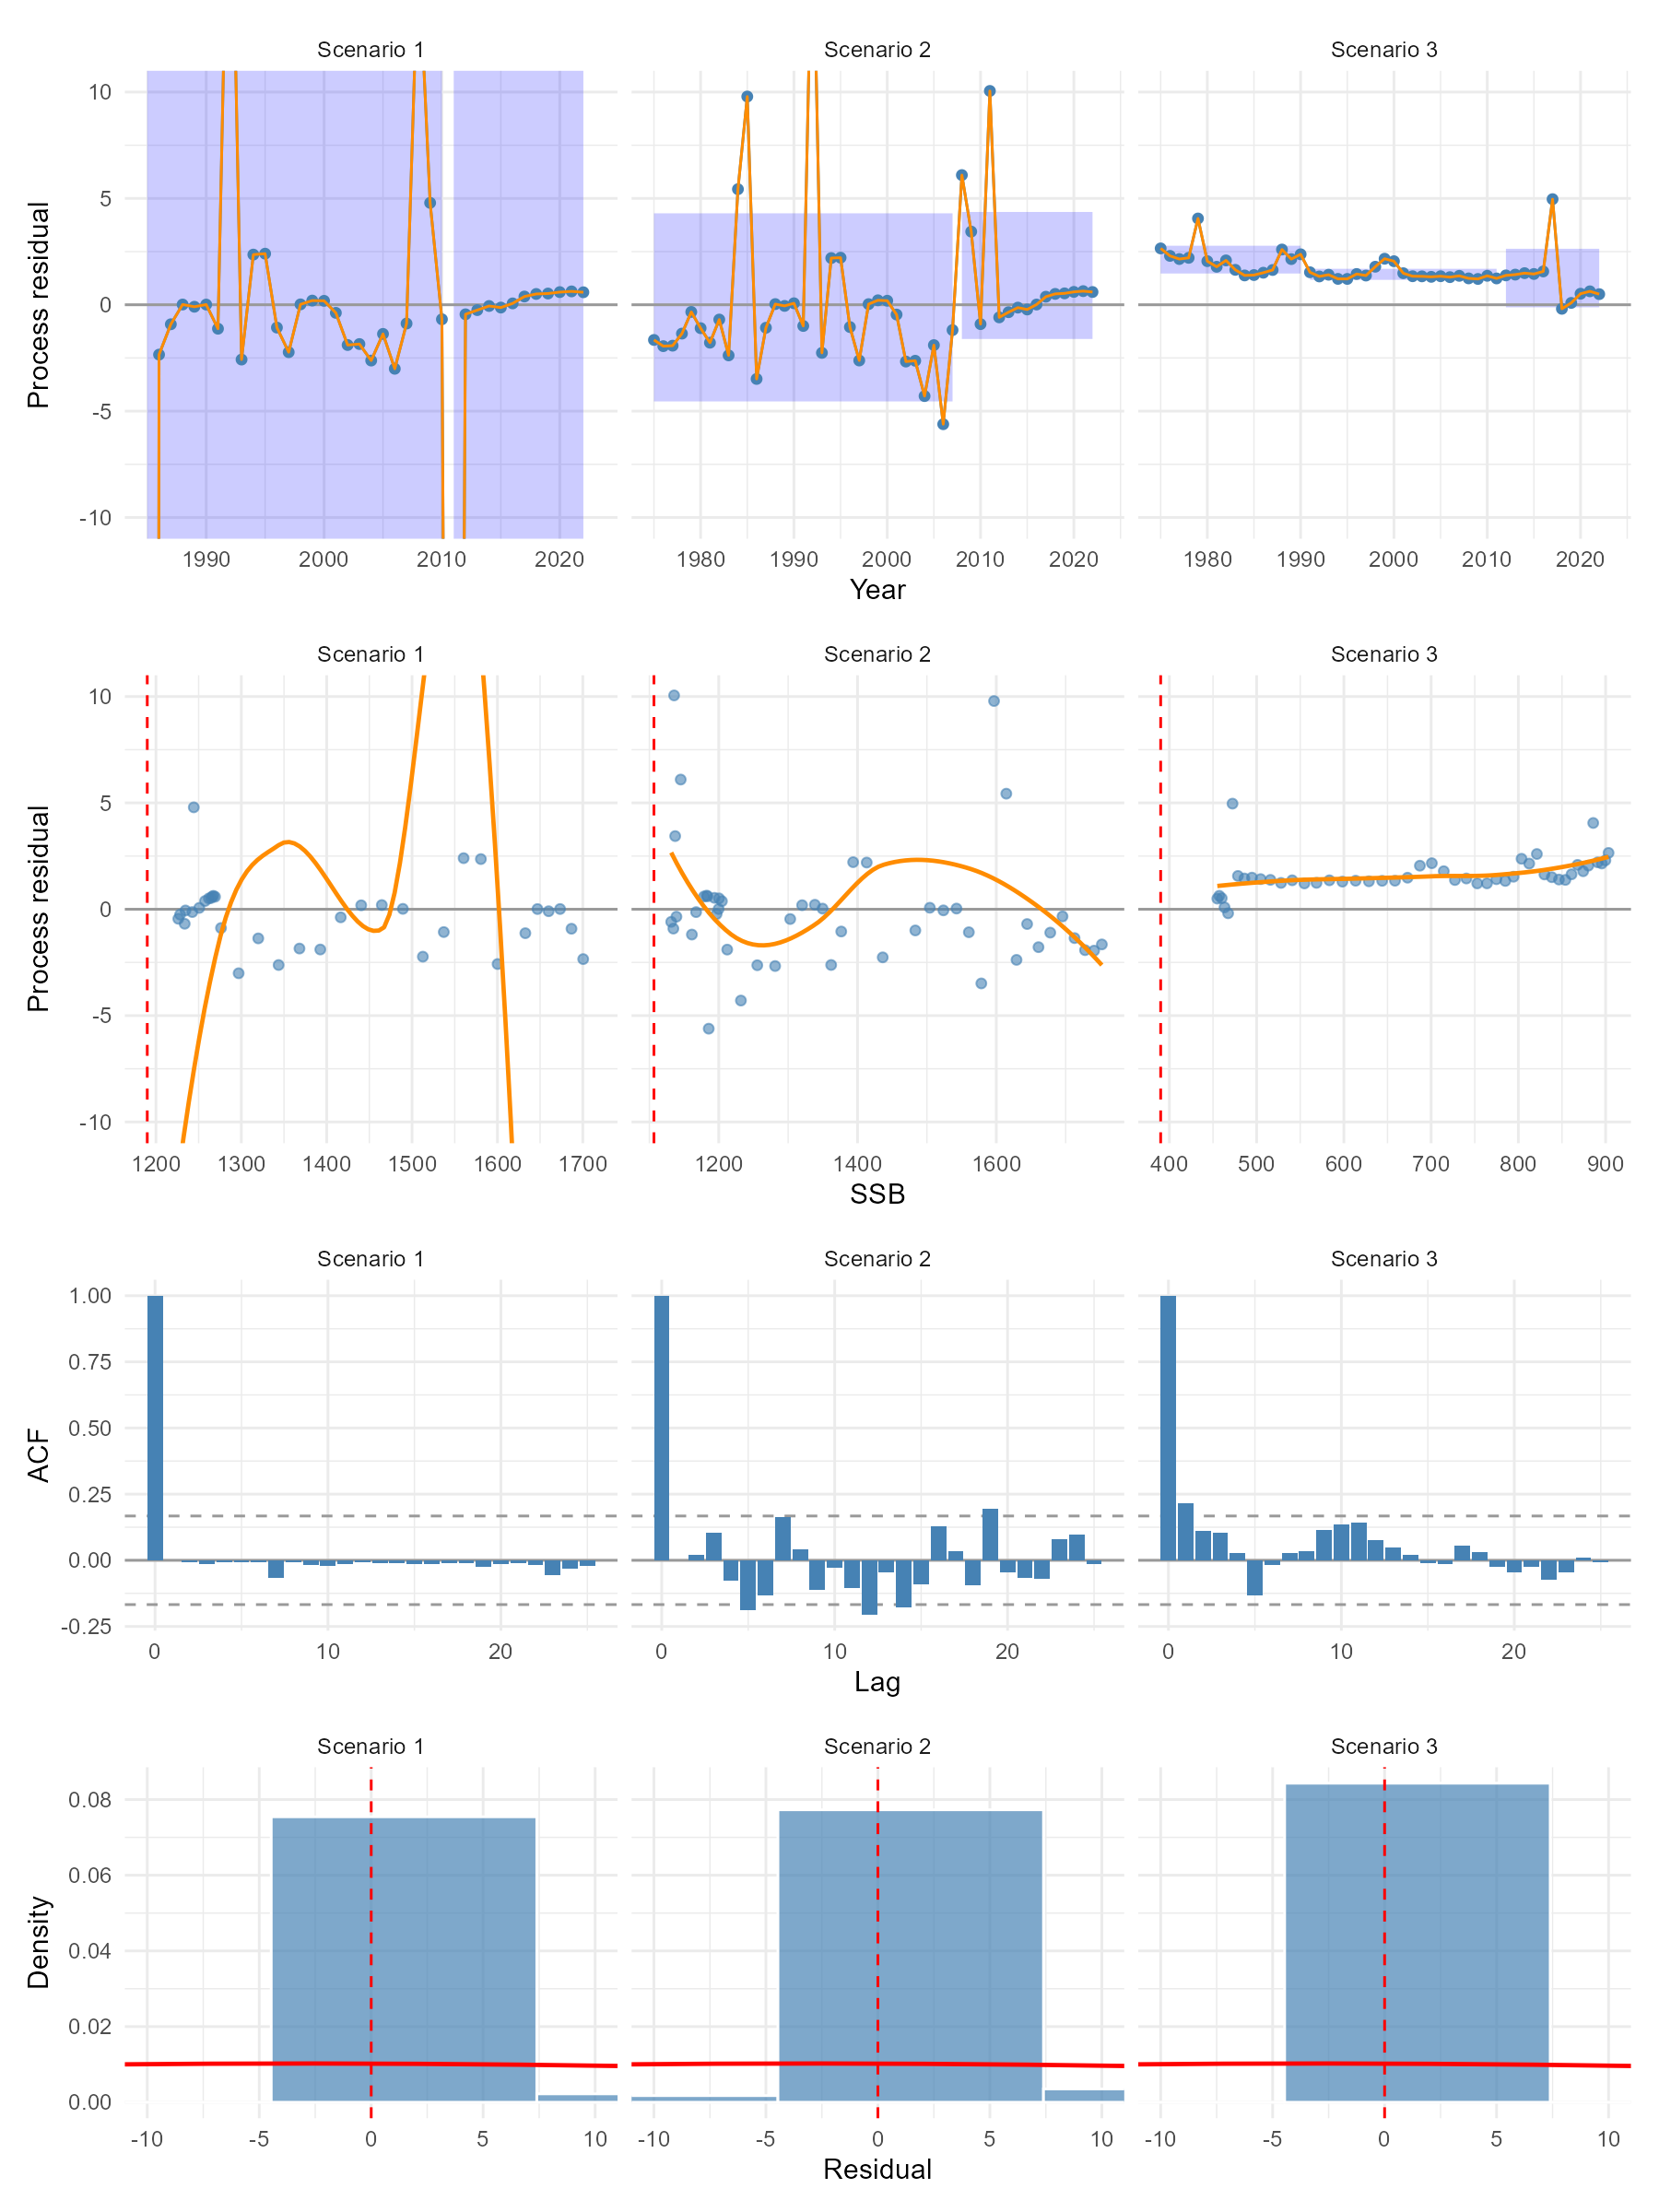
\includegraphics[width=0.92\linewidth]{figs/4panel.png}
  \caption{4panel}
  \label{fig:internal-4panel}
\end{figure}



\subsection{Interpretation}

Summarise whether the model is technically well fitted, which quantities are weakly
identified, and which issues should be carried forward to the robustness appendix.

% Case-specific internal interpretation.
% Summarise whether management quantities are informed by data,
% whether likelihood profiles or Hessian checks indicate weak identifiability,
% and which issues should be carried to the robustness appendix.



\section{External Diagnostics and Reproducible Workflow}
\label{app:external}

External diagnostics evaluate whether model outputs are consistent with specified
evidence outside the fitted likelihood. In this appendix, ``consistent'' should be
defined against explicit data sources or biological constraints, rather than by informal
judgement. Generic code for reading, plotting, and comparing indicators should live in
packages; case-study scripts should map model outputs to external evidence and write
results into the content files below.

\subsection{Required R Packages}

\begin{table}

\caption{\label{tab:external-libraries}Required R packages for external diagnostics.}
\centering
\begin{tabular}[t]{llll}
\toprule
package & role & tier & installed\\
\midrule
knitr & Knit template; format LaTeX tables & core & 1.51\\
r4ss & Read SS3 output for maturity, selectivity, and index fit & run\_code & 1.53.0\\
sstruth & diagSS, spSsbFromSs3, ssPeDiagnose; external CPUE and SP plots & run\_code & 0.0.0.9020\\
FLRebuild & curveSS(); production and reference points from SS3 & run\_code & 0.1.0\\
ss3om & readTruth / readFLSss3(); FLR stock objects from SS3 & run\_code & 0.5.3.9004\\
\addlinespace
FLCandy & matSel(); maturity vs selectivity ogives & run\_code & 1.7.1\\
diags & Extract CPUE/index series from SS3 diagnostics (.diagUss) & run\_code & 2.2.1\\
mpb & Lowess smoothing and scaling for CPUE time-series plots & run\_code & 3.5.0\\
plyr & Reshape index data (ddply) & run\_code & 1.8.9\\
reshape2 & Wide format for correlation plots (cast) & run\_code & 1.4.5\\
\addlinespace
ggplot2 & CPUE time series, survey vs biomass, sel/mat, LBI & run\_code & 4.0.3\\
GGally & Pairwise scatter plots of index correlations (planned) & planned & 2.4.0\\
ggcorrplot & Correlation matrix with hierarchical clustering (planned) & planned & 0.1.4.1\\
FLCore & FLR indicators and survey standardisation objects (planned) & planned & 2.6.29.9001\\
FLife & Cross-correlations between indices (planned) & planned & 3.4.0\\
\addlinespace
mydas & Life-history indicators (LBI); my\_smooth for ggpairs (planned) & planned & 1.2.2\\
\bottomrule
\end{tabular}
\end{table}



\subsection{Evidence Outside the Likelihood}

List the external evidence used in the case study:

\begin{itemize}
  \item life-history information, including growth, maturity, natural mortality, and longevity;
  \item fishery-independent survey trends, spatial indicators, and availability information;
  \item fishery behaviour, selectivity evidence, discard or bycatch information;
  \item environmental or ecosystem drivers already used in index standardisation;
  \item demographic indicators such as mature fraction, older-fish indicators, or age structure.
\end{itemize}

\begin{table}

\caption{\label{tab:external-evidence}External evidence register for the shortfin mako SS3 case study.}
\centering
\begin{tabular}[t]{lllll}
\toprule
diagnostic & evidence\_source & model\_quantity & criterion & status\\
\midrule
Growth and maturity & Life-history inputs to SS3 & Maturity-at-age vs selectivity-at-age & Fishing should not heavily precede 50 percent maturity on SSB scale & Check\\
Selectivity at age & Fleet selectivity ogives from SS3 & Selectivity ogive & Selectivity peak below maturity implies lagged SSB response & Mismatch flagged in case study\\
Survey perception & Standardised CPUE / survey indices (external to likelihood if pre-processed) & Index fit and scaling & Assessment trend coherent with survey perception & Check\\
Age structure & Length and age composition data & Age composition residuals & Older-fish / age-structure signals consistent with depletion narrative & Check\\
Spatial availability & Spatial models / availability (if used outside SS3) & Recruitment / availability deviations & No double-counting of spatial signal inside SS3 & Check\\
\addlinespace
Fishery behaviour / non-retention & Discard and non-retention regulations & Catch-at-age and discard mortality & Removals dominated by juveniles while state is mature female SSB & Mismatch flagged in case study\\
\bottomrule
\end{tabular}
\end{table}



\subsection{Standard Checks}

For SS3 and other age-structured assessments, useful external checks include maturity
versus selectivity, survey trend versus assessment biomass, spatial occupancy or aggregation
indicators, and comparison of recruitment or productivity regimes with external evidence.

% External comparison tables.

\begin{table}

\caption{\label{tab:external-sspe}Surplus-production vs SS3 process-error diagnostics (sstruth::ssPeDiagnose).}
\centering
\begin{tabular}[t]{lrrrrrrrl}
\toprule
scenario & curve\_cor & curve\_rmse & curve\_rel\_rmse & pe\_cor\_ssb & pe\_cor\_biomass & pe\_rmse\_ssb & pe\_rmse\_biomass & likely\_misspecified\\
\midrule
Scenario 1 & 0.9933 & 374.4 & 0.1159 & -0.2136 & 0.2427 & 7.196 & 0.006521 & TRUE\\
\bottomrule
\end{tabular}
\end{table}



\subsection{Diagnostic Output}

Tables, figures, and code-generated summaries can be added to the file below as they
become available.

% External diagnostic figures.

\begin{figure}[H]
  \centering
  \includegraphics[width=0.72\linewidth]{appendices/figs/external/cpue-ts.png}
  \caption{Standardised CPUE time series by fleet (sstruth::diagSS; lowess trend when mpb available).}
  \label{fig:external-cpue-ts}
\end{figure}

\begin{figure}[H]
  \centering
  \includegraphics[width=0.88\linewidth]{appendices/figs/external/sp-ssb.png}
  \caption{Empirical surplus production vs spawning stock biomass (sstruth::spSsbFromSs3).}
  \label{fig:external-sp-ssb}
\end{figure}

\begin{figure}[H]
  \centering
  \includegraphics[width=0.88\linewidth]{appendices/figs/external/selmat.png}
  \caption{Comparison of selectivity and maturity-at-age in the shortfin mako SS3 scenarios (from readFLSss3).}
  \label{fig:external-selmat}
\end{figure}



\subsection{Interpretation}

State which model outputs are consistent with external evidence, which are not, and which
external conflicts should be tested in the robustness appendix.

% Case-specific external interpretation.
% State which model outputs are consistent with life history and fishery evidence,
% which conflicts should be tested in the robustness appendix,
% and whether the biomass currency matches the age classes removed by fishing.



\section{Robustness Diagnostics and Reproducible Workflow}
\label{app:robustness}

Robustness diagnostics evaluate whether advice-relevant conclusions are stable under
pre-specified alternative structures. This appendix should separate estimation uncertainty
conditional on a reference model from sensitivity across models or scenarios. Generic
scenario comparison, hindcast, ensemble, and projection code should live in packages;
case-study scripts should define scenarios and write results into the content files below.

\subsection{Required R Packages}

\begin{table}

\caption{\label{tab:robustness-libraries}Required R packages for robustness diagnostics.}
\centering
\begin{tabular}[t]{llll}
\toprule
package & role & tier & installed\\
\midrule
knitr & Knit template; format LaTeX tables & core & 1.51\\
r4ss & Read SS3 output across scenarios & run\_code & 1.53.0\\
FLRebuild & curveSS(); scenario time series and process residuals & run\_code & 0.1.0\\
ss3om & readTruth / readFLSss3(); FLR stock objects from SS3 & run\_code & 0.5.3.9004\\
sstruth & retroBacktestData, plotRatios, ssPeDiagnose, plotSpSsb & run\_code & 0.0.0.9020\\
\addlinespace
ggplot2 & Scenario comparison, retrospective, and MVLN figures & run\_code & 4.0.3\\
dplyr & Retrospective trajectory plots (trajMsyLong); MVLN time-series summaries & run\_code & 1.2.1\\
plyr & Summarise scenario outputs (ddply) & run\_code & 1.8.9\\
reshape2 & Reshape scenario tables and MVLN draws (melt/cast) & run\_code & 1.4.5\\
tidyr & Reshape scenario and ensemble tables (planned) & planned & 1.3.2\\
\addlinespace
FLCore & FLR stock objects for status and reference points (planned) & planned & 2.6.29.9001\\
kobe & Kobe-phase plots (planned; ggplot used for MVLN Kobe comparison) & planned & 2.2.0\\
mvtnorm & Multivariate normal sampling for MVLN status uncertainty & run\_code & 1.3.3\\
patchwork & Combine MVLN status time-series panels (optional) & run\_code & 1.3.2\\
\bottomrule
\end{tabular}
\end{table}



\subsection{Scenario Register}

Each robustness appendix should begin with a scenario register. Scenarios should be
pre-specified before reviewing the results, and should identify which uncertainty source
they test.

\begin{table}

\caption{\label{tab:robustness-scenarios}Scenario register for robustness diagnostics (2026 ICCAT shark WG base runs).}
\centering
\begin{tabular}[t]{llllr}
\toprule
scenario & class & purpose & include\_in\_ensemble & weight\\
\midrule
Scenario 1 & reference & Reference assessment (Sc1\_Base) & TRUE & 0.3333333\\
Scenario 2 & structural sensitivity & Alternative structural assumption 1 (Scn02\_base) & TRUE & 0.3333333\\
Scenario 3 & structural sensitivity & Alternative structural assumption 2 (Sc3\_Base) & TRUE & 0.3333333\\
\bottomrule
\end{tabular}
\end{table}


\subsection{Standard Checks}

Robustness reporting should include:

\begin{itemize}
  \item retrospective patterns and hindcast or cross-validation prediction skill;
  \item alternative stock--recruitment, natural mortality, selectivity, catchability, or data-weighting structures;
  \item scenario or ensemble summaries for stock status, reference points, and catch advice;
  \item comparison of model error with estimation error from the reference case;
  \item central tendencies for target reference points and tail probabilities for limit reference points;
  \item rebuilding quantities such as $B_{\mathrm{rebuild}}$, $T_{\mathrm{rebuild}}$, and $P(\mathrm{rebuild\ within\ }T)$ where relevant;
  \item comparison of process-error diagnostics across model classes when ensembles combine biomass-dynamic (JABBA, SPiCT) and age-structured (SS3, SAM) formulations, using a common surplus-production currency on spawning biomass;
  \item hindcast and catch back-test forecast skill where retrospective peels are available.
\end{itemize}

% Robustness diagnostic checks.

\begin{table}

\caption{\label{tab:robustness-pe-summary}Terminal-year scenario status relative to MSY reference points (from curveSS).}
\centering
\begin{tabular}[t]{lrrrr}
\toprule
scenario & terminal\_year & ssb\_bmsy & catch\_msy & harvest\_fmsy\\
\midrule
Scenario 1 & 2023 & 1.07 & 0.429 & 0.401\\
Scenario 2 & 2023 & 1.07 & 0.436 & 0.408\\
Scenario 3 & 2023 & 1.16 & 0.742 & 0.639\\
\bottomrule
\end{tabular}
\end{table}

\begin{table}

\caption{\label{tab:robustness-sspe}Surplus-production misspecification flags by scenario (sstruth::ssPeDiagnose).}
\centering
\begin{tabular}[t]{lrrrrrrrl}
\toprule
scenario & curve\_cor & curve\_rmse & curve\_rel\_rmse & pe\_cor\_ssb & pe\_cor\_biomass & pe\_rmse\_ssb & pe\_rmse\_biomass & likely\_misspecified\\
\midrule
Scenario 1 & 0.9933 & 374.4 & 0.11590 & -0.21360 & 0.2427 & 7.196 & 0.006521 & TRUE\\
Scenario 2 & 0.9816 & 241.1 & 0.07565 & -0.06222 & -0.1129 & 16.800 & 0.007235 & TRUE\\
Scenario 3 & 0.9992 & 1200.0 & 0.64210 & 0.11780 & -0.2070 & 22.950 & 0.007739 & TRUE\\
\bottomrule
\end{tabular}
\end{table}

\begin{table}

\caption{\label{tab:robustness-retro-onestep}One-step-ahead retrospective errors (sstruth::retroBacktestData).}
\centering
\begin{tabular}[t]{llrrlrrrrrrrr}
\toprule
scenario & peel & terminalYr & forecastYr & baseRefEra & catchFore & forecastF & catchEstBaseTime & estFBaseTime & catchReportedData & relErrCatchVsEst & relErrFVsEst & relErrCatchVsReported\\
\midrule
Scenario-2 & 0 & 2023 & 2024 & FORE & 3497 & 0.18070 & 3497 & 0.1807 & 0 & 0.000000 & 0.000000 & NA\\
Scenario-2 & -1 & 2023 & 2024 & FORE & 3246 & 0.18230 & 3497 & 0.1807 & 0 & -0.071670 & 0.008362 & NA\\
Scenario-2 & -2 & 2023 & 2024 & FORE & 0 & 0.00000 & 3497 & 0.1807 & 0 & -1.000000 & -1.000000 & NA\\
Scenario-2 & -3 & 2023 & 2024 & FORE & 3582 & 0.19100 & 3497 & 0.1807 & 0 & 0.024420 & 0.056510 & NA\\
Scenario-2 & -4 & 2023 & 2024 & FORE & 3602 & 0.18690 & 3497 & 0.1807 & 0 & 0.030090 & 0.034030 & NA\\
\addlinespace
Scenario-2 & -5 & 2023 & 2024 & FORE & 3589 & 0.18030 & 3497 & 0.1807 & 0 & 0.026320 & -0.002669 & NA\\
Scenario-2 & -6 & 2023 & 2024 & FORE & 3577 & 0.17500 & 3497 & 0.1807 & 0 & 0.022840 & -0.032010 & NA\\
Scenario-2 & -7 & 2023 & 2024 & FORE & 3557 & 0.17460 & 3497 & 0.1807 & 0 & 0.017130 & -0.033830 & NA\\
Scenario-2 & -8 & 2023 & 2024 & FORE & 3470 & 0.17310 & 3497 & 0.1807 & 0 & -0.007715 & -0.042290 & NA\\
Scenario-2 & -9 & 2023 & 2024 & FORE & 3440 & 0.17280 & 3497 & 0.1807 & 0 & -0.016330 & -0.044060 & NA\\
\addlinespace
Scenario-2 & -10 & 2023 & 2024 & FORE & 3455 & 0.17330 & 3497 & 0.1807 & 0 & -0.011900 & -0.041230 & NA\\
Scenario-3 & 0 & 2023 & 2024 & FORE & 2056 & 0.08000 & 2056 & 0.0800 & 0 & 0.000000 & 0.000000 & NA\\
Scenario-3 & -1 & 2023 & 2024 & FORE & 0 & 0.00000 & 2056 & 0.0800 & 0 & -1.000000 & -1.000000 & NA\\
Scenario-3 & -2 & 2023 & 2024 & FORE & 1896 & 0.08577 & 2056 & 0.0800 & 0 & -0.077730 & 0.072210 & NA\\
Scenario-3 & -3 & 2023 & 2024 & FORE & 2032 & 0.08570 & 2056 & 0.0800 & 0 & -0.011440 & 0.071250 & NA\\
\addlinespace
Scenario-3 & -4 & 2023 & 2024 & FORE & 1927 & 0.08428 & 2056 & 0.0800 & 0 & -0.062570 & 0.053610 & NA\\
Scenario-3 & -5 & 2023 & 2024 & FORE & 1856 & 0.08289 & 2056 & 0.0800 & 0 & -0.097490 & 0.036150 & NA\\
Scenario-3 & -6 & 2023 & 2024 & FORE & 1780 & 0.08138 & 2056 & 0.0800 & 0 & -0.134400 & 0.017320 & NA\\
Scenario-3 & -7 & 2023 & 2024 & FORE & 1806 & 0.08284 & 2056 & 0.0800 & 0 & -0.121600 & 0.035590 & NA\\
Scenario-3 & -8 & 2023 & 2024 & FORE & 1722 & 0.08392 & 2056 & 0.0800 & 0 & -0.162600 & 0.049080 & NA\\
\addlinespace
Scenario-3 & -9 & 2023 & 2024 & FORE & 1542 & 0.08266 & 2056 & 0.0800 & 0 & -0.250200 & 0.033260 & NA\\
Scenario-3 & -10 & 2023 & 2024 & FORE & 1507 & 0.08584 & 2056 & 0.0800 & 0 & -0.267200 & 0.073090 & NA\\
\bottomrule
\end{tabular}
\end{table}

\begin{table}

\caption{\label{tab:robustness-mvln-terminal}Terminal-year MVLN status uncertainty by scenario (year 2023). Harvest = F/FMSY from Hessian draws.}
\centering
\begin{tabular}[t]{llrrrrrrrrrr}
\toprule
  & scenario & terminal\_year & stock\_median & stock\_p05 & stock\_p95 & harvest\_median & harvest\_p05 & harvest\_p95 & p\_overfished & p\_overfishing & weight\\
\midrule
Scenario-1 & Scenario-1 & 2023 & 1.05 & 0.867 & 1.32 & 24.3 & 21.0 & 27.9 & 0.326 & 1 & 0.333\\
Scenario-2 & Scenario-2 & 2023 & 1.06 & 0.926 & 1.22 & 25.4 & 23.1 & 28.1 & 0.220 & 1 & 0.333\\
Scenario-3 & Scenario-3 & 2023 & 1.16 & 0.938 & 1.42 & 43.3 & 35.5 & 52.7 & 0.112 & 1 & 0.333\\
\bottomrule
\end{tabular}
\end{table}

\begin{table}

\caption{\label{tab:robustness-catch-backtest}Catch back-test forecast summaries by peel and forecast scenario (collected via run-catch-backtests.R).}
\centering
\begin{tabular}[t]{lllrrrrll}
\toprule
scenario & peel & forecast\_scenario & forecast\_year & spawn\_bio & dead\_catch & sum\_f & run\_dir & ok\\
\midrule
Scenario-2 & 0 & catchReported & 2024 & 1188.0 & NA & NA & C:/active/flr/sstruth/data/ss3/sma-natl/Scenario-2/retrospectives/retro0/catchReported & TRUE\\
Scenario-2 & 0 & fMeanFull & 2024 & 1188.0 & NA & NA & C:/active/flr/sstruth/data/ss3/sma-natl/Scenario-2/retrospectives/retro0/fMeanFull & TRUE\\
Scenario-2 & 0 & fZero & 2024 & 1188.0 & NA & NA & C:/active/flr/sstruth/data/ss3/sma-natl/Scenario-2/retrospectives/retro0/fZero & TRUE\\
Scenario-2 & 0 & fMsy & 2024 & 1188.0 & NA & NA & C:/active/flr/sstruth/data/ss3/sma-natl/Scenario-2/retrospectives/retro0/fMsy & TRUE\\
Scenario-2 & -1 & catchReported & 2024 & 1184.0 & NA & NA & C:/active/flr/sstruth/data/ss3/sma-natl/Scenario-2/retrospectives/retro-1/catchReported & TRUE\\
\addlinespace
Scenario-2 & -1 & fMeanFull & 2024 & 1184.0 & NA & NA & C:/active/flr/sstruth/data/ss3/sma-natl/Scenario-2/retrospectives/retro-1/fMeanFull & TRUE\\
Scenario-2 & -1 & fZero & 2024 & 1184.0 & NA & NA & C:/active/flr/sstruth/data/ss3/sma-natl/Scenario-2/retrospectives/retro-1/fZero & TRUE\\
Scenario-2 & -1 & fMsy & 2024 & 1184.0 & NA & NA & C:/active/flr/sstruth/data/ss3/sma-natl/Scenario-2/retrospectives/retro-1/fMsy & TRUE\\
Scenario-2 & -2 & catchReported & 2024 & 1243.0 & NA & NA & C:/active/flr/sstruth/data/ss3/sma-natl/Scenario-2/retrospectives/retro-2/catchReported & TRUE\\
Scenario-2 & -2 & fMeanFull & 2024 & 1243.0 & NA & NA & C:/active/flr/sstruth/data/ss3/sma-natl/Scenario-2/retrospectives/retro-2/fMeanFull & TRUE\\
\addlinespace
Scenario-2 & -2 & fZero & 2024 & 1243.0 & NA & NA & C:/active/flr/sstruth/data/ss3/sma-natl/Scenario-2/retrospectives/retro-2/fZero & TRUE\\
Scenario-2 & -2 & fMsy & 2024 & 1243.0 & NA & NA & C:/active/flr/sstruth/data/ss3/sma-natl/Scenario-2/retrospectives/retro-2/fMsy & TRUE\\
Scenario-2 & -3 & catchReported & 2024 & 1252.0 & NA & NA & C:/active/flr/sstruth/data/ss3/sma-natl/Scenario-2/retrospectives/retro-3/catchReported & TRUE\\
Scenario-2 & -3 & fMeanFull & 2024 & 1252.0 & NA & NA & C:/active/flr/sstruth/data/ss3/sma-natl/Scenario-2/retrospectives/retro-3/fMeanFull & TRUE\\
Scenario-2 & -3 & fZero & 2024 & 1252.0 & NA & NA & C:/active/flr/sstruth/data/ss3/sma-natl/Scenario-2/retrospectives/retro-3/fZero & TRUE\\
\addlinespace
Scenario-2 & -3 & fMsy & 2024 & 1252.0 & NA & NA & C:/active/flr/sstruth/data/ss3/sma-natl/Scenario-2/retrospectives/retro-3/fMsy & TRUE\\
Scenario-2 & -4 & catchReported & 2024 & 1238.0 & NA & NA & C:/active/flr/sstruth/data/ss3/sma-natl/Scenario-2/retrospectives/retro-4/catchReported & TRUE\\
Scenario-2 & -4 & fMeanFull & 2024 & 1238.0 & NA & NA & C:/active/flr/sstruth/data/ss3/sma-natl/Scenario-2/retrospectives/retro-4/fMeanFull & TRUE\\
Scenario-2 & -4 & fZero & 2024 & 1238.0 & NA & NA & C:/active/flr/sstruth/data/ss3/sma-natl/Scenario-2/retrospectives/retro-4/fZero & TRUE\\
Scenario-2 & -4 & fMsy & 2024 & 1238.0 & NA & NA & C:/active/flr/sstruth/data/ss3/sma-natl/Scenario-2/retrospectives/retro-4/fMsy & TRUE\\
\addlinespace
Scenario-2 & -5 & catchReported & 2024 & 1203.0 & NA & NA & C:/active/flr/sstruth/data/ss3/sma-natl/Scenario-2/retrospectives/retro-5/catchReported & TRUE\\
Scenario-2 & -5 & fMeanFull & 2024 & 1203.0 & NA & NA & C:/active/flr/sstruth/data/ss3/sma-natl/Scenario-2/retrospectives/retro-5/fMeanFull & TRUE\\
Scenario-2 & -5 & fZero & 2024 & 1203.0 & NA & NA & C:/active/flr/sstruth/data/ss3/sma-natl/Scenario-2/retrospectives/retro-5/fZero & TRUE\\
Scenario-2 & -5 & fMsy & 2024 & 1203.0 & NA & NA & C:/active/flr/sstruth/data/ss3/sma-natl/Scenario-2/retrospectives/retro-5/fMsy & TRUE\\
Scenario-2 & -6 & catchReported & 2024 & 1196.0 & NA & NA & C:/active/flr/sstruth/data/ss3/sma-natl/Scenario-2/retrospectives/retro-6/catchReported & TRUE\\
\addlinespace
Scenario-2 & -6 & fMeanFull & 2024 & 1196.0 & NA & NA & C:/active/flr/sstruth/data/ss3/sma-natl/Scenario-2/retrospectives/retro-6/fMeanFull & TRUE\\
Scenario-2 & -6 & fZero & 2024 & 1196.0 & NA & NA & C:/active/flr/sstruth/data/ss3/sma-natl/Scenario-2/retrospectives/retro-6/fZero & TRUE\\
Scenario-2 & -6 & fMsy & 2024 & 1196.0 & NA & NA & C:/active/flr/sstruth/data/ss3/sma-natl/Scenario-2/retrospectives/retro-6/fMsy & TRUE\\
Scenario-2 & -7 & catchReported & 2024 & 1160.0 & NA & NA & C:/active/flr/sstruth/data/ss3/sma-natl/Scenario-2/retrospectives/retro-7/catchReported & TRUE\\
Scenario-2 & -7 & fMeanFull & 2024 & 1160.0 & NA & NA & C:/active/flr/sstruth/data/ss3/sma-natl/Scenario-2/retrospectives/retro-7/fMeanFull & TRUE\\
\addlinespace
Scenario-2 & -7 & fZero & 2024 & 1160.0 & NA & NA & C:/active/flr/sstruth/data/ss3/sma-natl/Scenario-2/retrospectives/retro-7/fZero & TRUE\\
Scenario-2 & -7 & fMsy & 2024 & 1160.0 & NA & NA & C:/active/flr/sstruth/data/ss3/sma-natl/Scenario-2/retrospectives/retro-7/fMsy & TRUE\\
Scenario-2 & -8 & catchReported & 2024 & 1116.0 & NA & NA & C:/active/flr/sstruth/data/ss3/sma-natl/Scenario-2/retrospectives/retro-8/catchReported & TRUE\\
Scenario-2 & -8 & fMeanFull & 2024 & 1116.0 & NA & NA & C:/active/flr/sstruth/data/ss3/sma-natl/Scenario-2/retrospectives/retro-8/fMeanFull & TRUE\\
Scenario-2 & -8 & fZero & 2024 & 1116.0 & NA & NA & C:/active/flr/sstruth/data/ss3/sma-natl/Scenario-2/retrospectives/retro-8/fZero & TRUE\\
\addlinespace
Scenario-2 & -8 & fMsy & 2024 & 1116.0 & NA & NA & C:/active/flr/sstruth/data/ss3/sma-natl/Scenario-2/retrospectives/retro-8/fMsy & TRUE\\
Scenario-2 & -9 & catchReported & 2024 & 1089.0 & NA & NA & C:/active/flr/sstruth/data/ss3/sma-natl/Scenario-2/retrospectives/retro-9/catchReported & TRUE\\
Scenario-2 & -9 & fMeanFull & 2024 & 1089.0 & NA & NA & C:/active/flr/sstruth/data/ss3/sma-natl/Scenario-2/retrospectives/retro-9/fMeanFull & TRUE\\
Scenario-2 & -9 & fZero & 2024 & 1089.0 & NA & NA & C:/active/flr/sstruth/data/ss3/sma-natl/Scenario-2/retrospectives/retro-9/fZero & TRUE\\
Scenario-2 & -9 & fMsy & 2024 & 1089.0 & NA & NA & C:/active/flr/sstruth/data/ss3/sma-natl/Scenario-2/retrospectives/retro-9/fMsy & TRUE\\
\addlinespace
Scenario-2 & -10 & catchReported & 2024 & 1079.0 & NA & NA & C:/active/flr/sstruth/data/ss3/sma-natl/Scenario-2/retrospectives/retro-10/catchReported & TRUE\\
Scenario-2 & -10 & fMeanFull & 2024 & 1079.0 & NA & NA & C:/active/flr/sstruth/data/ss3/sma-natl/Scenario-2/retrospectives/retro-10/fMeanFull & TRUE\\
Scenario-2 & -10 & fZero & 2024 & 1079.0 & NA & NA & C:/active/flr/sstruth/data/ss3/sma-natl/Scenario-2/retrospectives/retro-10/fZero & TRUE\\
Scenario-2 & -10 & fMsy & 2024 & 1079.0 & NA & NA & C:/active/flr/sstruth/data/ss3/sma-natl/Scenario-2/retrospectives/retro-10/fMsy & TRUE\\
Scenario-3 & 0 & catchReported & 2024 & 451.1 & NA & NA & C:/active/flr/sstruth/data/ss3/sma-natl/Scenario-3/retrospectives/retro0/catchReported & TRUE\\
\addlinespace
Scenario-3 & 0 & fMeanFull & 2024 & 451.1 & NA & NA & C:/active/flr/sstruth/data/ss3/sma-natl/Scenario-3/retrospectives/retro0/fMeanFull & TRUE\\
Scenario-3 & 0 & fZero & 2024 & 451.1 & NA & NA & C:/active/flr/sstruth/data/ss3/sma-natl/Scenario-3/retrospectives/retro0/fZero & TRUE\\
Scenario-3 & 0 & fMsy & 2024 & 451.1 & NA & NA & C:/active/flr/sstruth/data/ss3/sma-natl/Scenario-3/retrospectives/retro0/fMsy & TRUE\\
Scenario-3 & -1 & catchReported & 2024 & 447.3 & NA & NA & C:/active/flr/sstruth/data/ss3/sma-natl/Scenario-3/retrospectives/retro-1/catchReported & TRUE\\
Scenario-3 & -1 & fMeanFull & 2024 & 447.3 & NA & NA & C:/active/flr/sstruth/data/ss3/sma-natl/Scenario-3/retrospectives/retro-1/fMeanFull & TRUE\\
\addlinespace
Scenario-3 & -1 & fZero & 2024 & 447.3 & NA & NA & C:/active/flr/sstruth/data/ss3/sma-natl/Scenario-3/retrospectives/retro-1/fZero & TRUE\\
Scenario-3 & -1 & fMsy & 2024 & 447.3 & NA & NA & C:/active/flr/sstruth/data/ss3/sma-natl/Scenario-3/retrospectives/retro-1/fMsy & TRUE\\
Scenario-3 & -2 & catchReported & 2024 & 472.4 & NA & NA & C:/active/flr/sstruth/data/ss3/sma-natl/Scenario-3/retrospectives/retro-2/catchReported & TRUE\\
Scenario-3 & -2 & fMeanFull & 2024 & 472.4 & NA & NA & C:/active/flr/sstruth/data/ss3/sma-natl/Scenario-3/retrospectives/retro-2/fMeanFull & TRUE\\
Scenario-3 & -2 & fZero & 2024 & 472.4 & NA & NA & C:/active/flr/sstruth/data/ss3/sma-natl/Scenario-3/retrospectives/retro-2/fZero & TRUE\\
\addlinespace
Scenario-3 & -2 & fMsy & 2024 & 472.4 & NA & NA & C:/active/flr/sstruth/data/ss3/sma-natl/Scenario-3/retrospectives/retro-2/fMsy & TRUE\\
Scenario-3 & -3 & catchReported & 2024 & 471.4 & NA & NA & C:/active/flr/sstruth/data/ss3/sma-natl/Scenario-3/retrospectives/retro-3/catchReported & TRUE\\
Scenario-3 & -3 & fMeanFull & 2024 & 471.4 & NA & NA & C:/active/flr/sstruth/data/ss3/sma-natl/Scenario-3/retrospectives/retro-3/fMeanFull & TRUE\\
Scenario-3 & -3 & fZero & 2024 & 471.4 & NA & NA & C:/active/flr/sstruth/data/ss3/sma-natl/Scenario-3/retrospectives/retro-3/fZero & TRUE\\
Scenario-3 & -3 & fMsy & 2024 & 471.4 & NA & NA & C:/active/flr/sstruth/data/ss3/sma-natl/Scenario-3/retrospectives/retro-3/fMsy & TRUE\\
\addlinespace
Scenario-3 & -4 & catchReported & 2024 & 463.6 & NA & NA & C:/active/flr/sstruth/data/ss3/sma-natl/Scenario-3/retrospectives/retro-4/catchReported & TRUE\\
Scenario-3 & -4 & fMeanFull & 2024 & 463.6 & NA & NA & C:/active/flr/sstruth/data/ss3/sma-natl/Scenario-3/retrospectives/retro-4/fMeanFull & TRUE\\
Scenario-3 & -4 & fZero & 2024 & 463.6 & NA & NA & C:/active/flr/sstruth/data/ss3/sma-natl/Scenario-3/retrospectives/retro-4/fZero & TRUE\\
Scenario-3 & -4 & fMsy & 2024 & 463.6 & NA & NA & C:/active/flr/sstruth/data/ss3/sma-natl/Scenario-3/retrospectives/retro-4/fMsy & TRUE\\
Scenario-3 & -5 & catchReported & 2024 & 448.2 & NA & NA & C:/active/flr/sstruth/data/ss3/sma-natl/Scenario-3/retrospectives/retro-5/catchReported & TRUE\\
\addlinespace
Scenario-3 & -5 & fMeanFull & 2024 & 448.2 & NA & NA & C:/active/flr/sstruth/data/ss3/sma-natl/Scenario-3/retrospectives/retro-5/fMeanFull & TRUE\\
Scenario-3 & -5 & fZero & 2024 & 448.2 & NA & NA & C:/active/flr/sstruth/data/ss3/sma-natl/Scenario-3/retrospectives/retro-5/fZero & TRUE\\
Scenario-3 & -5 & fMsy & 2024 & 448.2 & NA & NA & C:/active/flr/sstruth/data/ss3/sma-natl/Scenario-3/retrospectives/retro-5/fMsy & TRUE\\
Scenario-3 & -6 & catchReported & 2024 & 436.5 & NA & NA & C:/active/flr/sstruth/data/ss3/sma-natl/Scenario-3/retrospectives/retro-6/catchReported & TRUE\\
Scenario-3 & -6 & fMeanFull & 2024 & 436.5 & NA & NA & C:/active/flr/sstruth/data/ss3/sma-natl/Scenario-3/retrospectives/retro-6/fMeanFull & TRUE\\
\addlinespace
Scenario-3 & -6 & fZero & 2024 & 436.5 & NA & NA & C:/active/flr/sstruth/data/ss3/sma-natl/Scenario-3/retrospectives/retro-6/fZero & TRUE\\
Scenario-3 & -6 & fMsy & 2024 & 436.5 & NA & NA & C:/active/flr/sstruth/data/ss3/sma-natl/Scenario-3/retrospectives/retro-6/fMsy & TRUE\\
Scenario-3 & -7 & catchReported & 2024 & 435.6 & NA & NA & C:/active/flr/sstruth/data/ss3/sma-natl/Scenario-3/retrospectives/retro-7/catchReported & TRUE\\
Scenario-3 & -7 & fMeanFull & 2024 & 435.6 & NA & NA & C:/active/flr/sstruth/data/ss3/sma-natl/Scenario-3/retrospectives/retro-7/fMeanFull & TRUE\\
Scenario-3 & -7 & fZero & 2024 & 435.6 & NA & NA & C:/active/flr/sstruth/data/ss3/sma-natl/Scenario-3/retrospectives/retro-7/fZero & TRUE\\
\addlinespace
Scenario-3 & -7 & fMsy & 2024 & 435.6 & NA & NA & C:/active/flr/sstruth/data/ss3/sma-natl/Scenario-3/retrospectives/retro-7/fMsy & TRUE\\
Scenario-3 & -8 & catchReported & 2024 & 415.5 & NA & NA & C:/active/flr/sstruth/data/ss3/sma-natl/Scenario-3/retrospectives/retro-8/catchReported & TRUE\\
Scenario-3 & -8 & fMeanFull & 2024 & 415.5 & NA & NA & C:/active/flr/sstruth/data/ss3/sma-natl/Scenario-3/retrospectives/retro-8/fMeanFull & TRUE\\
Scenario-3 & -8 & fZero & 2024 & 415.5 & NA & NA & C:/active/flr/sstruth/data/ss3/sma-natl/Scenario-3/retrospectives/retro-8/fZero & TRUE\\
Scenario-3 & -8 & fMsy & 2024 & 415.5 & NA & NA & C:/active/flr/sstruth/data/ss3/sma-natl/Scenario-3/retrospectives/retro-8/fMsy & TRUE\\
\addlinespace
Scenario-3 & -9 & catchReported & 2024 & 380.5 & NA & NA & C:/active/flr/sstruth/data/ss3/sma-natl/Scenario-3/retrospectives/retro-9/catchReported & TRUE\\
Scenario-3 & -9 & fMeanFull & 2024 & 380.5 & NA & NA & C:/active/flr/sstruth/data/ss3/sma-natl/Scenario-3/retrospectives/retro-9/fMeanFull & TRUE\\
Scenario-3 & -9 & fZero & 2024 & 380.5 & NA & NA & C:/active/flr/sstruth/data/ss3/sma-natl/Scenario-3/retrospectives/retro-9/fZero & TRUE\\
Scenario-3 & -9 & fMsy & 2024 & 380.5 & NA & NA & C:/active/flr/sstruth/data/ss3/sma-natl/Scenario-3/retrospectives/retro-9/fMsy & TRUE\\
Scenario-3 & -10 & catchReported & 2024 & 356.2 & NA & NA & C:/active/flr/sstruth/data/ss3/sma-natl/Scenario-3/retrospectives/retro-10/catchReported & TRUE\\
\addlinespace
Scenario-3 & -10 & fMeanFull & 2024 & 356.2 & NA & NA & C:/active/flr/sstruth/data/ss3/sma-natl/Scenario-3/retrospectives/retro-10/fMeanFull & TRUE\\
Scenario-3 & -10 & fZero & 2024 & 356.2 & NA & NA & C:/active/flr/sstruth/data/ss3/sma-natl/Scenario-3/retrospectives/retro-10/fZero & TRUE\\
Scenario-3 & -10 & fMsy & 2024 & 356.2 & NA & NA & C:/active/flr/sstruth/data/ss3/sma-natl/Scenario-3/retrospectives/retro-10/fMsy & TRUE\\
\bottomrule
\end{tabular}
\end{table}



\subsection{Diagnostic Output}

Tables, figures, and code-generated summaries can be added to the file below as they
become available.

% Robustness diagnostic figures.

\begin{figure}[H]
  \centering
  \includegraphics[width=0.92\linewidth]{appendices/figs/robustness/ss3-ts.png}
  \caption{SS3 scenario time series relative to MSY reference points.}
  \label{fig:robustness-ss3-ts}
\end{figure}

\begin{figure}[H]
  \centering
  \includegraphics[width=0.92\linewidth]{appendices/figs/robustness/ss3-res-time.png}
  \caption{Process residuals by scenario (from curveSS).}
  \label{fig:robustness-ss3-res-time}
\end{figure}

\begin{figure}[H]
  \centering
  \includegraphics[width=0.92\linewidth]{appendices/figs/robustness/ss3-res-acf.png}
  \caption{ACF of process residuals by scenario.}
  \label{fig:robustness-ss3-res-acf}
\end{figure}

\begin{figure}[H]
  \centering
  \includegraphics[width=0.95\linewidth]{appendices/figs/robustness/retro-traj-msy.png}
  \caption{Retrospective peel trajectories vs MSY benchmarks (sstruth::retroBacktestData).}
  \label{fig:robustness-retro-traj}
\end{figure}

\begin{figure}[H]
  \centering
  \includegraphics[width=0.92\linewidth]{appendices/figs/robustness/retro-bratio-horizon.png}
  \caption{Multi-horizon SSB/BMSY retrospective ratios (sstruth::plotRatios).}
  \label{fig:robustness-retro-bratio}
\end{figure}

\begin{figure}[H]
  \centering
  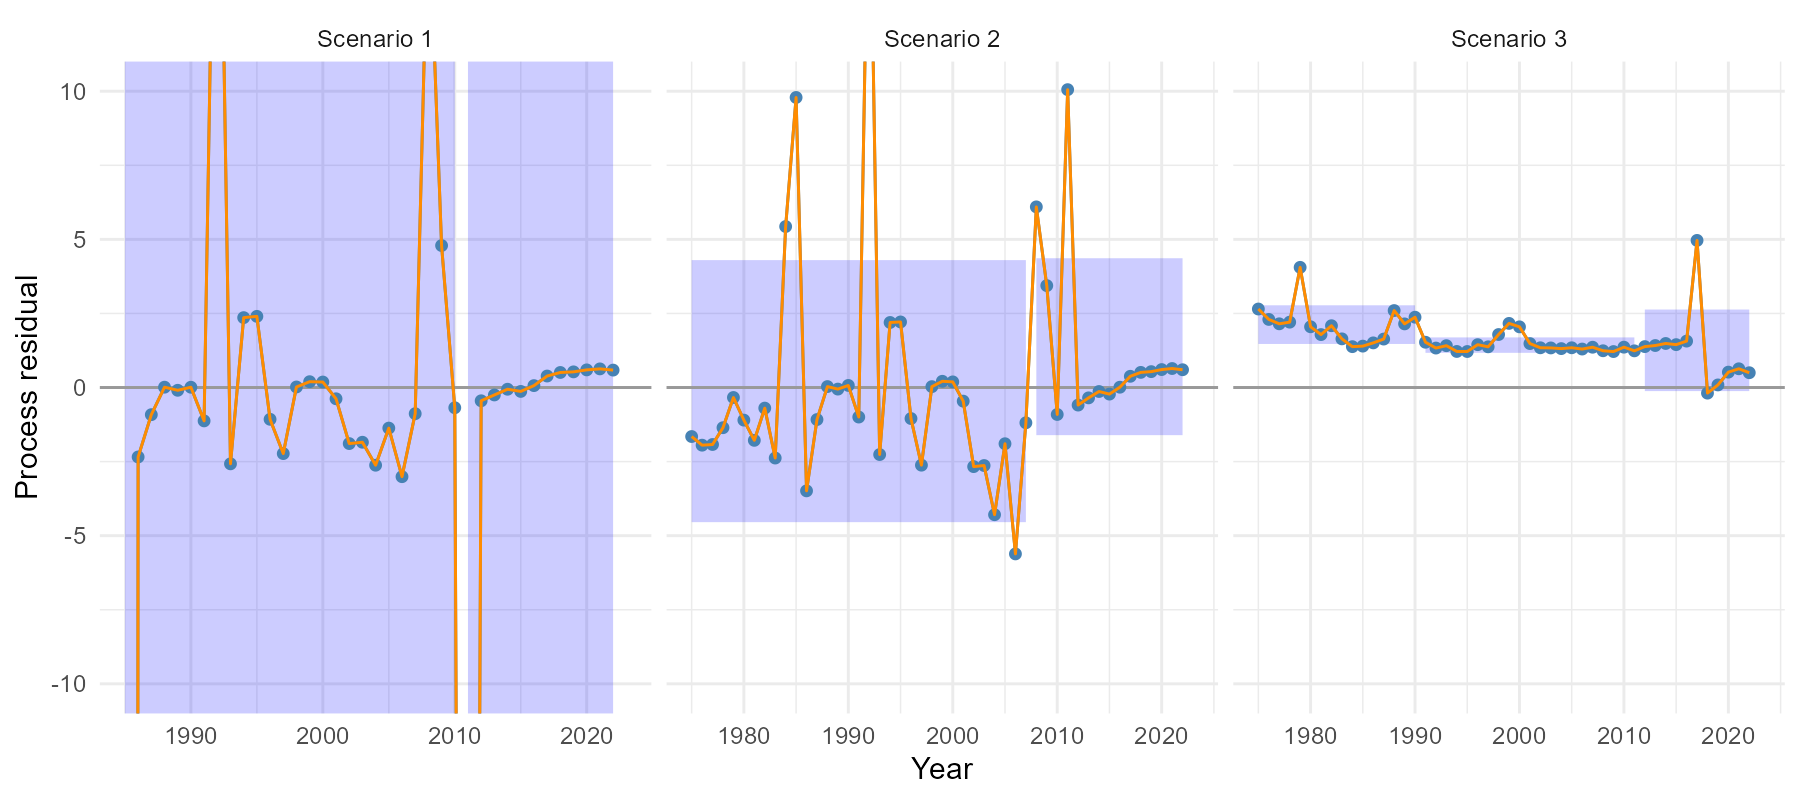
\includegraphics[width=0.92\linewidth]{figs/sma-fig-res-time-1.png}
  \caption{sma fig res time 1}
  \label{fig:robustness-sma-fig-res-time-1}
\end{figure}

\begin{figure}[H]
  \centering
  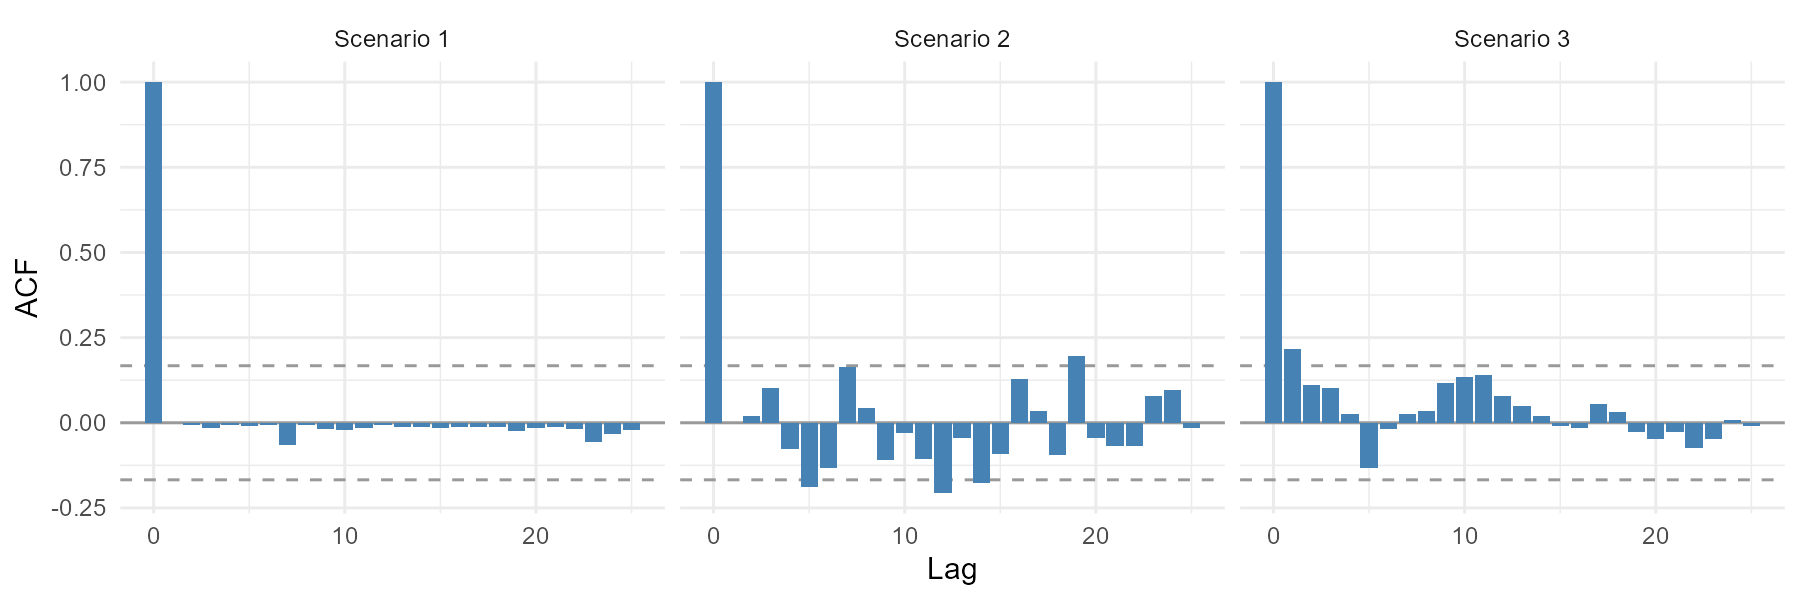
\includegraphics[width=0.92\linewidth]{figs/sma-fig-res-acf-1.png}
  \caption{sma fig res acf 1}
  \label{fig:robustness-sma-fig-res-acf-1}
\end{figure}



\subsection{Best Assessment Versus Ensemble}

If the estimates from pre-specified alternative models remain within the uncertainty
intervals of the reference model for the management quantities of interest, a best
assessment may be adequate for advice. If model sensitivity is larger than estimation
uncertainty, especially for limit tail probabilities or target central tendencies, advice is
model-dependent and should be reported using a scenario set or ensemble.

% Best-assessment versus ensemble comparison (MVLN).

% Reference scenario: Scenario-1; MVLN Monte Carlo draws = 500 per scenario.

\begin{table}

\caption{\label{tab:robustness-mvln-ensemble}MVLN terminal status and tail probabilities (year 2023). Compare estimation uncertainty (reference) with structural sensitivity scenarios.}
\centering
\begin{tabular}[t]{llrrrrrrrrrr}
\toprule
  & scenario & terminal\_year & stock\_median & stock\_p05 & stock\_p95 & harvest\_median & harvest\_p05 & harvest\_p95 & p\_overfished & p\_overfishing & weight\\
\midrule
Scenario-1 & Scenario-1 & 2023 & 1.05 & 0.867 & 1.32 & 24.3 & 21.0 & 27.9 & 0.326 & 1 & 0.333\\
Scenario-2 & Scenario-2 & 2023 & 1.06 & 0.926 & 1.22 & 25.4 & 23.1 & 28.1 & 0.220 & 1 & 0.333\\
Scenario-3 & Scenario-3 & 2023 & 1.16 & 0.938 & 1.42 & 43.3 & 35.5 & 52.7 & 0.112 & 1 & 0.333\\
\bottomrule
\end{tabular}
\end{table}

\begin{table}

\caption{\label{tab:robustness-ensemble-weight-comparison}Ensemble weight comparison by scenario: (i) equal weights; (ii) ICES-style Akaike weights $w_i \propto \exp(-\Delta\mathrm{AIC}/2)$ from total SS3 negative log-likelihood (comparable models); (iii) CVindexmase; (iv) CVindexrho (hindcast skill from retrospective peels; Scenarios 2--3 only until LOO CPUE is collected).}
\centering
\begin{tabular}[t]{lrrrr}
\toprule
scenario & w\_equal & w\_ices & w\_cvindexmase & w\_cvindexrho\\
\midrule
Scenario-1 & 0.3333 & 0 & NA & NA\\
Scenario-2 & 0.3333 & 1 & 1 & 0.6667\\
Scenario-3 & 0.3333 & 0 & 0 & 0.3333\\
\bottomrule
\end{tabular}
\end{table}

\begin{figure}[H]
  \centering
  \includegraphics[width=0.92\linewidth]{appendices/figs/robustness/mvln-kobe-terminal.png}
  \caption{Terminal-year Kobe-style comparison of MVLN draws: reference (Scenario-1) vs structural sensitivity scenarios.}
  \label{fig:robustness-mvln-kobe}
\end{figure}

\begin{figure}[H]
  \centering
  \includegraphics[width=0.92\linewidth]{appendices/figs/robustness/mvln-terminal-compare.png}
  \caption{Terminal MVLN medians and 5--95\% intervals for SSB/BMSY and F/FMSY by scenario.}
  \label{fig:robustness-mvln-terminal}
\end{figure}

\begin{figure}[H]
  \centering
  \includegraphics[width=0.92\linewidth]{appendices/figs/robustness/mvln-status-ts.png}
  \caption{Recent-year MVLN status trajectories with 5--95\% intervals by scenario.}
  \label{fig:robustness-mvln-ts}
\end{figure}



\subsection{Interpretation}

State which advice quantities are robust, which are model-dependent, and whether the
case study should be presented as a best assessment, a screened scenario set, an ensemble,
or an MSE operating-model set.

% Case-specific robustness interpretation.
% State which advice quantities are robust, which are model-dependent,
% and whether reporting should use a best assessment, screened scenario set, or ensemble.




\bibliographystyle{plainnat}
\bibliography{refs}

\end{document}
